% ------------------------------------------------
% Nomenclature list - update if needed
\nomenclature[G]{$\mathcal{D}$}{A dataset}
\nomenclature[G]{$\P$}{A probability distribution}
\nomenclature[G]{SOTA}{State of the Art}
\nomenclature[G]{RNN}{Recurrent Neural Network}
\nomenclature[G]{LSTM}{Long Short Term Memory (Network/Architecture)}
\nomenclature[G]{(T)ABSA}{(Target) Aspect Based Sentiment Analysis}
\nomenclature[G]{LM}{Language Model}
\nomenclature[G]{QA}{Question Answering}
\nomenclature[G]{NER}{Named Entity Recognition}
\nomenclature[G]{NLI}{Natural Language Inference - e.g similarity of two sentences or next sentence prediction task}
\nomenclature[G]{NLU}{Natural Language Understanding}
\nomenclature[G]{GLUE}{General Language Understanding Evaluation benchmark - a common set of tasks for which we train, evaluate and analyse NLU systems}
\nomenclature[G]{Support}{We adopt the mathematical definition of support: the number of nonzero points in a domain. In our case, it will refer to the number of instances of examples.}

\nomenclature[L]{ELMo}{Embeddings from Language Models}
\nomenclature[L]{GPT}{Generalised Pre Training}
\nomenclature[L]{RoBERTa}{Robustly optimised BERT approach}

\nomenclature[Z]{$\mathcal{S}$}{Support Set}
\nomenclature[Z]{$\mathcal{Q}$}{Query Set}
% ------------------------------------------------
\chapter{Background} \label{chapter:background}
In this chapter, we give a slightly expanded history of the field of NLP, referencing the evolution of language models building up to the current state of the art (SOTA) models used in this thesis. The critical analyses of the literature review will occur primarily on these works, while the preceding sections act as a prelude. Further, we analyse the field of multitask learning applied to language models, with particular focus on the Sentiment Analysis task, and the more granular Aspect Based Sentiment Analysis (ABSA) task that we will be focusing on in the experimentation element of this thesis.

To be consistent throughout this section, we define a \textit{parameter} of a model as a (set of) number(s) that can be learned directly during the training process - e.g a set of weights or biases - whereas a \textit{hyperparameter} cannot be learned directly during training, but has to be defined \textit{a priori} from the user. These hyperparameters will affect the performance of the model, and typically a (grid or random) search is conducted over some reasonable space in order to optimise what these numbers should be.

\section{The Evolution of Language Modelling}
The goal of this section is to outline various methodologies that lead to us modelling language. Our goal is to find some word representation vector that summarises a word in a given context; i.e. representation learning. We ideally want the word vectors of similar words, such as ``hotel" and ``motel" to be roughly equivalent ($\mathbf{w}_\text{hotel} \approx \mathbf{w}_\text{motel} \Rightarrow \mathbf{w}_\text{hotel} \cdot \mathbf{w}_\text{motel} \approx 1$) since they are used in similar contexts to represent similar things. Learning high quality representations can be challenging, since ideally we should model both the complex characteristics of word use (e.g., syntax and semantics), and how these uses vary across linguistic contexts (i.e. to model polysemy).
\subsection{Problem Setup} \label{section:background:problemsetup}
To formally define the language modelling setup: our goal is to infer a probability distribution $\P$ that predicts the next word given the \textit{context}. For now, the context will refer to all previous words, but we will explore subsets of previous words and surrounding words as contexts in sections \ref{section:background:ngram} and \ref{section:background:bidirectional}. That is, at time $t$ we want to predict word $\mathbf{w}_{t+1}$ given words $\mathbf{w}_{1:t} = \{ \mathbf{w}_1, \dots, \mathbf{w}_t \}$. Each word comes from a vocabulary $V$, so that $\forall i: \mathbf{w}_i \in V = \{\mathbf{w}^{(1)}, \dots, \mathbf{w}^{(|V|)}\} $.

By Bayes Rule, we may write that
\begin{align}
\P(\mathbf{w}_{t+1} | \mathbf{w}_{1:t}) = \frac{\P(\mathbf{w}_{1:(t+1)})}{\P(\mathbf{w}_{1:t})} \approx \frac{\text{count}(\mathbf{w}_{1:(t+1)})}{\text{count}(\mathbf{w}_{1:t})}
\end{align} 
where $\text{count}(\mathbf{w}_{1:i})$ refers to the number of instances of the strings containing $\mathbf{w}_1 \land \dots \land \mathbf{w}_i$ in some (ideally large) corpus of text. Note the commutitivity of the logical \texttt{OR} operation means that sequential structure is not preserved. In addition, this approximation does not scale well with $t$ since the prediction of words given a large context require good counts of very specific long strings in order to get meaningful approximation to the probability, which are unlikely to appear exactly in the corpus. This approach is thus computationally intractable and data inefficient. These can also be referred to as storage and sparsity problems respectively.

\subsection{$n-$gram models} \label{section:background:ngram}
To deal with data inefficiency, we can make a natural simplification that the \textit{context} is not the entire preceding string, but instead the previous $n-1$ words for some chosen (hyperparameter) $n$. The concatenation of $n$ words is called an ``$n-$gram" \cite{Brown}. Clearly, the larger the value of $n$ the more context we have, but the more data inefficient the procedure is as we encounter the same problem as before with the specific $n-$gram being unlikely to appear in our text corpus frequently. The lower the value of $n$ means we are disregarding increasing amounts of contextual information, so this represents a tradeoff for researchers. In practice, often 2-grams (``{{\color{red} bi}grams") and 3-grams (``{{\color{red} tri}grams") are used.

However, we still encounter the sparsity problem. If our $n-$gram in the numerator does not exist in the corpus then our probability distribution would predict that word having probability 0 of occuring, meaning we are biasing our distribution towards the particular corpus(es) used. A partial solution to this is adding some $\varepsilon$ to every word $\mathbf{w} \in V$, called \textit{smoothing}. If the $(n-1)$-gram in the denominator does not exist then our approximate probability distribution is not well defined, but a partial solution is to instead \textit{backoff} to the maximal $(n-k)-$gram that does exist in the corpus. These partial solutions do not fix the overall problem that $n-$gram models tend to exhibit reasonable local structure, but fail to capture long term dependencies and relationships to have any global meaning. We need a smarter model, and one that balances this important interplay between non trivial contextual information and data efficiency.


\subsection{Pretrained Word Embeddings: Humble Beginnings} \label{section:background:wordembeddings}

In the previous sections, we have described the importance of context to language modelling. The first class of methods that ignited research into word embeddings and representations was the Word2Vec models by Google \cite{Mikolov}. They built upon the Skip Gram model \cite{Mikolov2013} to learn distributed vector representations that captured syntactic and semantic word relationships, and proposed extensions that could be applied to the Continuous Bag Of Words (CBOW) model which they also introduced, as seen in Figure \ref{fig:background:SkipGramvsCBOW}. In particular, they introduced some key training techniques such as negative sampling and hierarchical softmax which enabled them to ingest orders of magnitude more training data from which greater amounts of contexts could be seen.

Despite the primitive neural network model, the word vectors are specifically trained to predict the surrounding words in the sentence via backpropagation to maximise the average log probability in a context window of size $c$ and thus the vectors can be seen as representing the distribution of context in which the word appears.

\begin{center}
	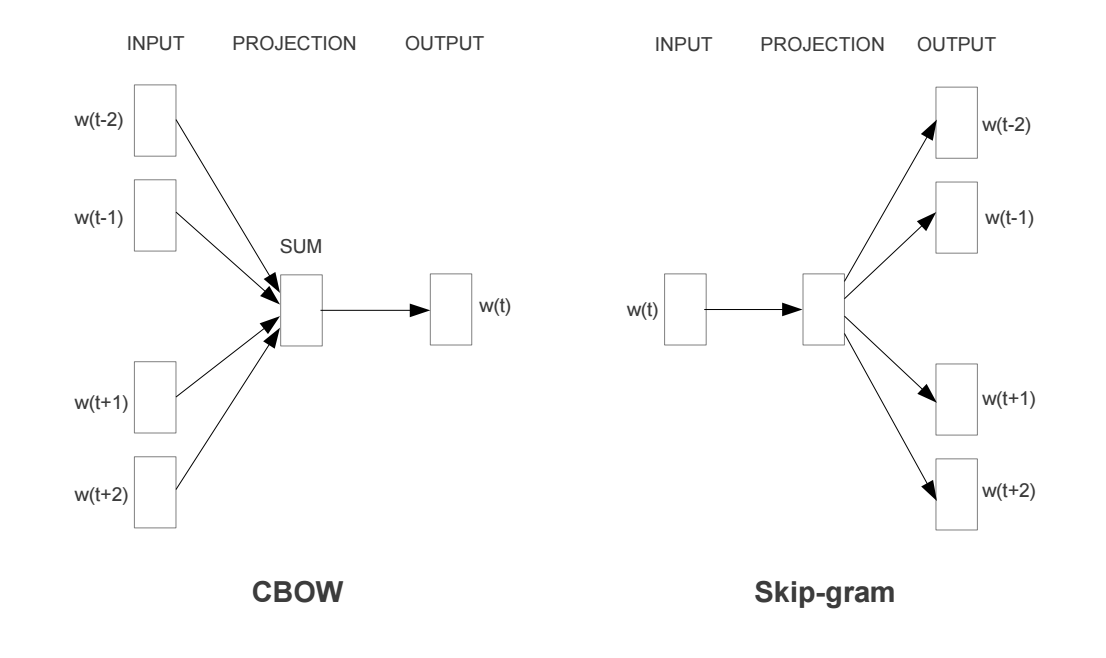
\includegraphics[width=.75\textwidth]{CBOWvsSkipGram.png}
	\captionof{figure}{Continuous Bag Of Word (CBOW) models vs Skip Gram Models \newline Skip Gram models predict a words context given the word itself, whereas CBOW models predict a word given its context.}
	\label{fig:background:SkipGramvsCBOW}
\end{center}

GloVe Vectors \cite{Pennington} take a different approach, and propose a weighted least squares model that looks to factorise the (log) word co-occurance matrix. They show that this approach can be formalised mathematically in the setting of an extension proposed by Mikolov \cite{Mikolov}, and do additional training tricks such as filtering the data to reduce the weighting factor for more frequent words during training (since these words appear in many contexts, and thus dont carry as much information).

Since the methods they proposed could ingest larger still amounts of context by leveraging age-old scalable mathematical optimsiation routines \cite{Pennington}, their results proved state of the art, as well as the fact that they were much more sample efficient, with accuracies around 4\% higher than the CBOW or Skip-Gram methods given the same compute time.

The important factor about these methods, is that the word embeddings captured contextual structure. We can look at a lower dimensional representation of the embedding space using dimensionality reduction techniques, for example tSNE \cite{VanDerMaaten2008}, which uses a stochastic neighbour embedding that aims to approximate the high dimensional structure in the form of a similarity matrix of conditional probabilities between datapoints with a lower dimensional onevoptimised by minimising the Kullback-Leibler Divergence \cite{Kullback1951}, to find that \textit{similar words occupy similar regions of the embedding space}. This indicates that the embedding space learned captures contextual information, since words close in the embedding space are ``associative neighbours" \footnote{in the linguistic sense, an associative neighbour $y$ of a word $x$ is a word such that when $x$ is replaced by $y$ in a given context, the sentence still makes sense.} - this is demonstrated in Figure \ref{fig:background:wordembeddings}. Interestingly, we can define an algebra in this space, in the sense that the relationship between clusters of words are represented by similar vectors (e.g tenses, but also more complex world information such as country-capital).

\begin{center}
	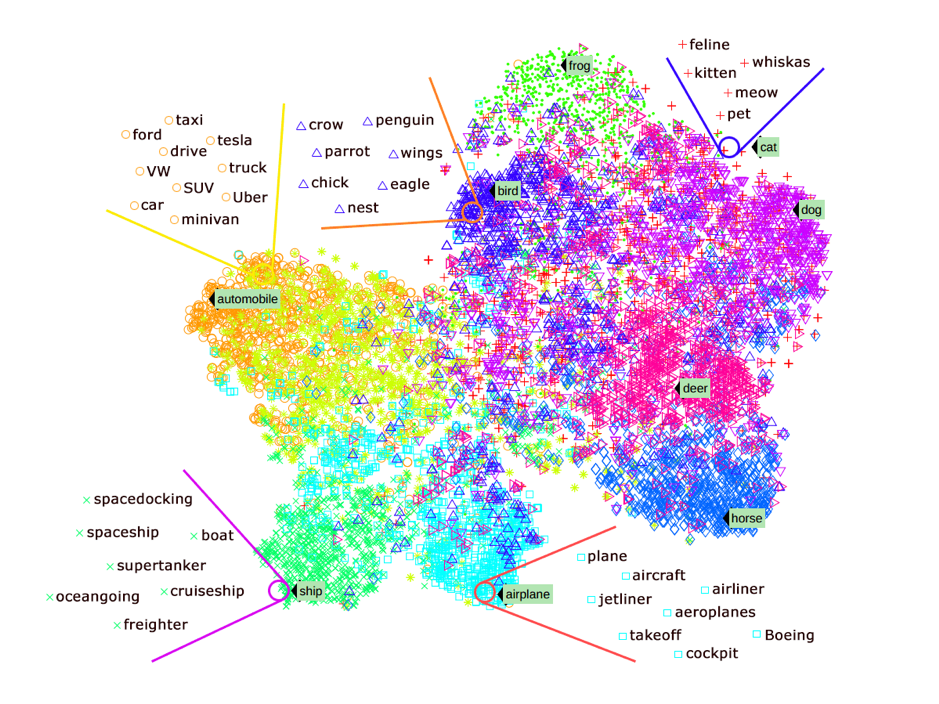
\includegraphics[width=.75\textwidth]{wordembeddings.png} \\
	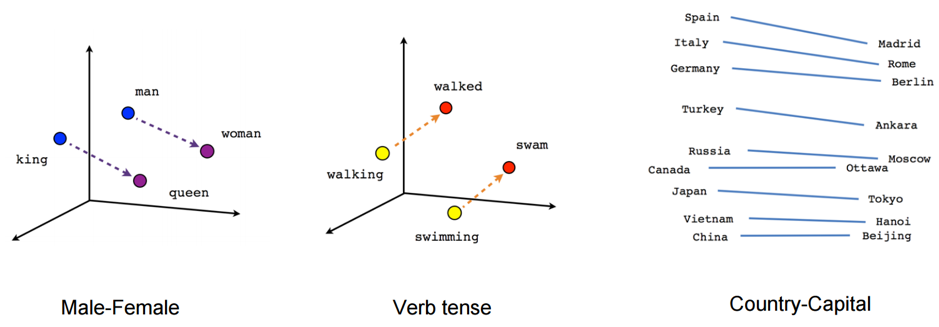
\includegraphics[width=.75\textwidth]{wordalgebra.png}
	\captionof{figure}{The reduced dimensionality word embedding space found using \texttt{word2vec} \cite{Mikolov} and the algebraic relationship between clusters of words in this space}
	\label{fig:background:wordembeddings}
\end{center}

\subsection{The Rise of Deep Learning: Using Sequentiality for Context} \label{section:background:bidirectional}
Deep learning successes tend to come in the large data regime. The distributional semantics hypothesis proposed by Saussure (as discussed in Section \ref{section:intro:history}) can apply directly here, since we simply need to ingest lots of data about how words are used and in which contexts and this is, in a sense, all we need to know about the word (e.g we don't need to form any external world view or model, a word is entirely defined by the contexts it is used in). The previous section highlights that word vectors are effective in capturing contextual information, and in this section we explore deeply uni/bi-directional models.

The disadvantage of the methods previously discussed is that it might be good to have a good representation for each word, but how do we combine them? As a baseline we could, once we have a good word representation, just ``average the words (embeddings)" to get a sentence embedding. This has its drawbacks, however, in that we lose the word order and sequentiality structure. We focus, now, on networks that take into account the sequential structure that gained traction in the field, that build upon these simply averaging/concatenation models of word embeddings to.

\subsubsection{Recurrent Neural Networks}
Recurrent Neural Networks \cite{Elman1990} are an ideal choice to deal with dynamic length input sequences that are prevalent in all NLP tasks. They are defined by two simple equations: RNNs store a hidden state representation at every timestep (which here corresponds to a word/token in the sentence) and they use this hidden state $\mathbf{h}_t$ to: (a) update its hidden state representation at the next time step whilst including information about the current time steps (i.e word) input and (b) make a prediction based on this hidden state at each time step. They are optimised using backpropagation through time \cite{Werbos}. For input $\mathbf{x}_t$ and hidden state $\mathbf{h}_t$ at time $t$, weight matrices $W_i$ and biases $\mathbf{b}_{\{h,o\}}$ we can get the prediction at time $t+1$, $\hat{\mathbf{y}}_{t+1}$ with the update rules:
\begin{align}
\mathbf{h}_{t+1} = \sigma \left(W_1 \mathbf{x}_{t+1} + W_2 \mathbf{h}_t + \mathbf{b}_h \right) \tag{a} \\
\hat{\mathbf{y}}_{t+1} = \text{softmax}\left(W_3 \mathbf{h}_{t+1} + \mathbf{b}_o \right) \tag{b}
\end{align}
 However, they suffered from vanishing and exploding gradient problems \cite{Pascanu}, where the backpropagation of the gradient through the network would prove in practice unstable, since the product of matrices unrolling through time can shrink to 0 or grow to infinity (along some direction $\mathbf{v}$) in value.

The proposed solution to this was introduced was a Long Short Term Memory (LSTM) Network \cite{Hochreiter1997}, which is similar to a RNN except the inclusion of gates which allow information to propagate through a ``cell". It keeps a hidden cell state of accumulated ``memory" and decides how much of the information from the next word in the sequence should be incorporated into its hidden state.

\begin{center}
	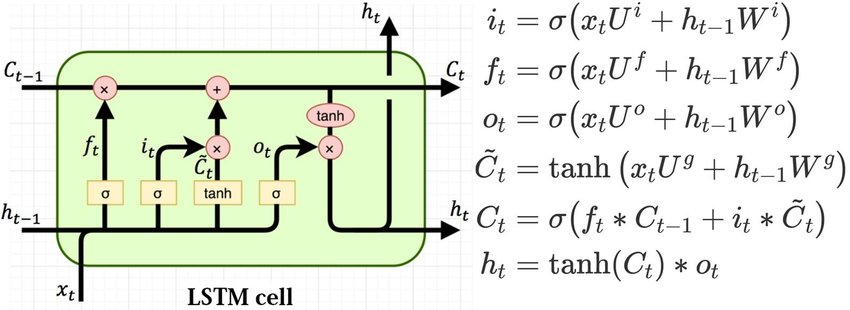
\includegraphics[width=.75\textwidth]{lstm.png}
	\captionof{figure}{One LSTM cell with corresponding equations, image taken from \cite{Varsamopoulos2018}. There is one cell for each word in the input sentence. We input embedding $x_t$, and propagate forward the hidden state $h_t$ and the cell state $C_t$. $\{i_t, f_t, o_t\}$ are the \{input, forget, output\} gates, $W^{\{i,f,o\}}$ and $U^{\{i,f,o\}}$ are learnable weight matrices.}
	\label{fig:background:lstm}
\end{center}

Following from this, Graves et al. showcased the power of Deep \textit{Bidirectional} LSTM (DBLSTM) networks for speech recognition temporal classification task \cite{Graves2013}. This small yet powerful modification allows the model to account for both sequential directions of context, and gives a much richer word representation since we can account for downstream words/tokens as opposed to just words/tokens seen prior to the current word at timestep $t$. It achieves this as per Figure \ref{fig:background:bidirectionallstm}, by implementing two LSTM models in parallel, one propagating forward through the input tokens and the other propagating backward through the input tokens, and concatenating together the hidden states of each model into a hidden state for the entire architecture. Then, inference is performed as above.

\begin{center}
	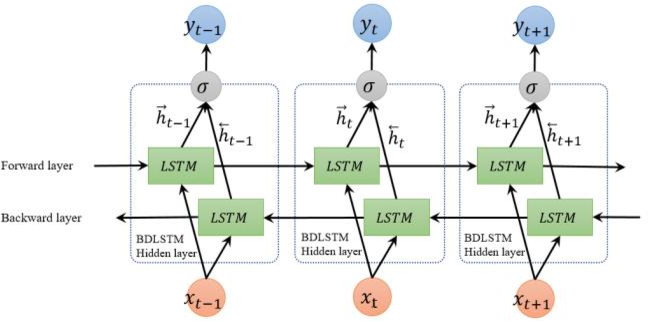
\includegraphics[width=.75\textwidth]{bidirectionallstm.png}
	\captionof{figure}{Bidirectional LSTM architecture as defined in \cite{Graves2013}}
	\label{fig:background:bidirectionallstm}
\end{center}

\subsubsection{ELMo \& GPT}
There have been many works to get rich context embeddings, but one of the most successful was ELMo \cite{Peters2018a} (\underline{E}mbeddings from \underline{L}anguage \underline{Mo}dels). Building upon the work of context dependent representations with bidirectional LSTM networks, ELMo embeddings utilise the DBLSTM architecture, but add regularisation and task specific weightings of all the hidden bidirectional layer represenations. Thus, unlike traditional word embeddings in Section \ref{section:background:wordembeddings}, the word representations are functions of the entire input sequence.

ELMo \cite{Peters2018a} proposes to extract context-sensitive features from a language model. OpenAI's GPT (Generalised Pre Training) Language Model \cite{RadfordGPT}, however, enhances the context-sensitive embedding by adjusting the Transformer architecture \cite{Vaswani}. Since the transformer architecture is utilised in the current state of the art models, treatment and analysis of this architecture is deferred to section \ref{section:background:LMs}. While the GPT Model did not outperform SOTA Sentiment Analysis, it achieved SOTA on 9 out of 12 NLP tasks, and provided an important stepping stone to the state of the art language models, showcasing the power of the TransformerXL \cite{Dai2019} architecture, which actually enables learning dependency beyond a fixed context width unlike the other recurrent models through having recurrent mechanisms inside the architecture focusing on certain ``segments". However, this is still a ``standard" language modelling setup in the sense that it is a unidirectional model. The importance of this paper was to set up the following paradigm: \textit{generative pre-training} of a language model on a diverse corpus of unlabeled text, followed by \textit{discriminative fine-tuning} on each specific downstream task. This is the paradigm we use throughout this thesis, and this paper first demonstrated its efficacy on a range of downstream tasks including absolute improvements of 8.9\% on commonsense reasoning tasks, 5.7\% on question answering tasks, and 1.5\% on textual entailment tasks.

\section{Current SOTA Language Modelling: Transformers} \label{section:background:LMs}
The previous section provides a basis of understanding on which the current state of the art models are built upon. We outlined important ideas of bidirectional context embeddings, and explore further in this section how state of the art language models have been built. These are the models that were implemented for our experiments (outlined in Chapter \ref{chapter:experiments}), and what we built additional functionality on top of.

Following the successes of inductive transfer learning applied to Computer Vision \cite{He2015, Huang2016}, where large convolutional and residual architectures were pretrained on large common image datasets such as ImageNet \cite{ImageNet} and COCO \cite{COCO}, focus was redirected onto training large pretrained models that would act as a Language Model. Up until this point, Deep Learning had showed promise in achieving state of the art on many different NLP tasks, but there was rarely a consistent model architecture (since researchers often hand crafted task specific architectures in order to achieve SOTA performance), and these models were often trained from scratch which required large datasets and days to converge. In 2018, researchers proposed Universal Language Model Fine-tuning (ULMFiT) \cite{Howard2018}, an effective transfer learning method that could be applied to any task in NLP, and introduced key techniques for fine-tuning a language model.

Their aim, as is common to all subsequent language model variants, was to define a model that was expressive enough to, in a sense, ``capture language" via a (set of) suitable pretraining task(s). Such a model could ingest large quantities of unlabelled text data, and learn ``good" (contextualised) word embeddings. Then, the classifier could be fine tuned (via subsequent linear layers) to capture the idiosyncracies of the downstream target task (especially if the target task was different from the pretraining task). This would require additional data, but the premise of transfer learning is that it requires orders of magnitude less training data than training a model from scratch, since it can leverage pre-existing knowledge in the form of the pretrained word embeddings \cite{RuderThesis}.
\subsection{Transformer Architecture}
While prior models relied on convolutional or recurrent architectures, in 2017 researchers proposed a novel architecture: the Transformer \cite{Vaswani}, based solely on \textit{attention mechanisms}, dispensing with recurrence and convolutions frameworks entirely. They found in experiments on two machine translation tasks that these models were superior in quality but, more importantly, they demonstrated the models ability to be more parallelizable and requiring significantly less time to train than previous models. This would allow for the ingestion of more data from which to learn in a given time frame and potentially yield much more powerful models.

\subsubsection{Attention: An Introduction}
Self-attention, sometimes called intra-attention, is an attention mechanism relating different positions of a single sequence in order to compute a representation of the sequence. Self-attention had been used successfully in a variety of tasks including reading comprehension, abstractive summarization, textual entailment and learning task-independent sentence representations prior to the Transformer network \cite{Cheng2016, Parikh, Paulus2017, Lin2017}, but the Transformer network was the first end-to-end transduction model relying entirely on self-attention to compute representations of its input and output without using any recurrent or convolution elements.

The reader is referred to the diagram in Figure \ref{fig:background:transformer} taken from the original paper, but we first describe all the components of the diagram in detail.

\subsubsection{Encoder and Decoder Architecture}
\textbf{Encoder:} The encoder is composed of a stack of $N$ identical layers, with two sub-layers: the first is a multi-head self-attention mechanism, and the second is a fully connected feed forward (linear) layer. The authors utilise a residual connection \cite{He2015} around each of the sublayers, as well as employing layer normalization \cite{Ba2016}. All sub-layers in the model, as well as the embedding layers, produce outputs of dimension $d_\text{model}$.

\noindent \textbf{Decoder:} The decoder is also composed of a stack of $N$ identical layers: as well as the two sub-layers in each encoder layer, the decoder inserts an additional third sub-layer, which performs multi-head attention over the output of the encoder stack. As before, the authors use residual connections around each of the sub-layers, followed by layer normalization. They also modify the self-attention sublayer in the decoder stack to prevent positions from attending to subsequent positions. They refer to this as \textit{masked self attention} and this, combined with fact that the output embeddings are offset by one position, ensures that the predictions for position $i$ can depend only on the known outputs at positions less than $i$ (i.e it cannot see itself or into the future).

\subsubsection{Attention: The Mathematical Formalism}
An attention function can be described as mapping a \textit{query} and a set of \textit{key-value} pairs to an \textit{output}, where the query, keys, values, and output are all vectors of dimensionalities $d_k, d_k, d_v, d_\text{model}$, respectively. The output is computed as a weighted sum of the values, where the weight assigned to each value is computed by a compatibility function of the query with the corresponding key.

The authors compute the attention function, which they called ``Scaled Dot Product Attention" on a set of queries simultaneously, packed together into a matrix $Q$. The keys and values are also packed together into matrices $K$ and $V$, respectively. Then, the matrix of outputs is computed as:
\begin{align*}
\text{Attention}(Q, K, V) = \text{softmax}\left( \frac{QK^T}{\sqrt{d_k}} \right) V
\end{align*}
where the inverse of the square root of $d_k$, the dimensionality of the keys (and also queries), provides a scaling factor since the dot product between the keys and the queries can get large. The first term provides ``attention weights" which determine the linear combination of the values $V$. In essence, we see how similar the query is to each of the keys, then take a corresponding simililarity weighted linear combination of the values corresponding to those keys.

Multi-headed attention allows the model to jointly attend to information from different representation subspaces at different positions, with the intuition that, as well as providing a form of regularisation to the model, the model can attend to ``different types of things in each head" since it forms a specific representation in each one. Formally, we can write:
\begin{align*}
\text{MultiHead}(Q,K, V) &= \text{Concat}(\text{head}_1, \dots, \text{head}_h) W^O \\
\text{where head}_i &= \text{Attention}(Q W_i^Q ,K W_i^K , V W_i^V )
\end{align*}

where the projections into each head subspace are parameter matrices:
\begin{align*}
W_i^Q \in \mathbb{R}^{d_\text{model} \times d_k} , W_i^K \in \mathbb{R}^{d_\text{model} \times d_k} , W_i^V \in \mathbb{R}^{d_\text{model} \times d_v} \text{ and } W^O \in \mathbb{R}^{h\cdot d_v \times d_\text{model}}
\end{align*}

\begin{center}
	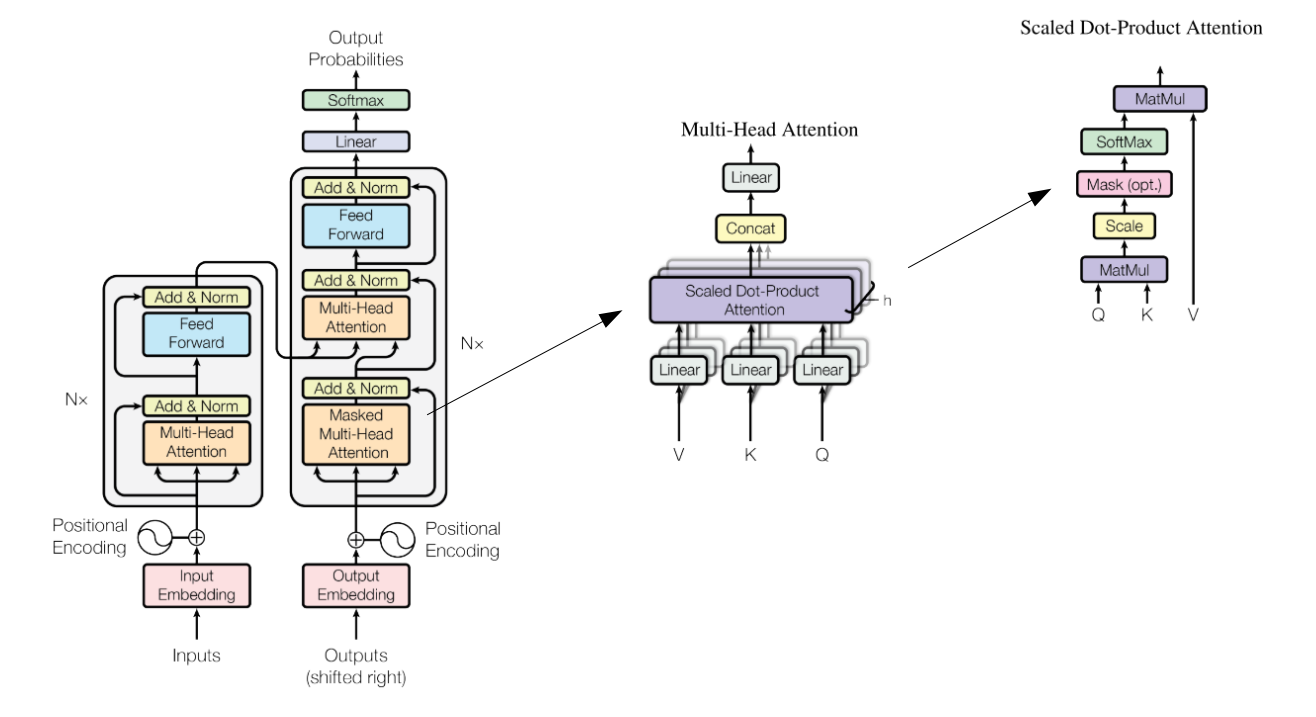
\includegraphics[width=\textwidth]{TransformerArchitecture.png}
	\captionof{figure}{The Architecture of the Transformer Model \cite{Vaswani}}
	\label{fig:background:transformer}
\end{center}

\subsubsection{Benefits of Self Attention}
There are many benefits of an end-to-end attention model over traditional recurrent or convolutional models, in particular the computational complexity per layer (compared in detail in Table 1 in \cite{Vaswani}), the amount of parallelisation computations (due to the lack of sequentiality needed - a major limitation identified in Section \ref{section:background:bidirectional})), and the path lengths the information has to travel in both forward backpropagation passes (of the gradients of the loss through the network) which can destabilise the learning procedure.

The authors note of an additional benefit: interpretability of models. They inspect attention distributions from their models and present and discuss examples in the appendix. They find that individual attention heads clearly learn to perform different tasks, many appear to exhibit behavior related to the syntactic and semantic structure of the sentences, although recent papers \cite{Jain} have disputed this claim having found that after running extensive experiments on a variety of NLP tasks, the attention distributions are uncorrelated with gradient-based measures of feature importance, and one can identify very different attention distributions that nonetheless yield equivalent predictions. Research in this area is ongoing, and outside the scope of this thesis.

\subsection{BERT} \label{section:background:bert}
\begin{center}
	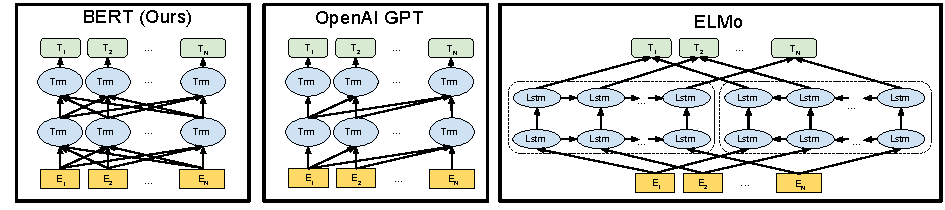
\includegraphics[width=\textwidth]{BERTvsELMovsGPT.pdf}
	\captionof{figure}{BERT vs OpenAI GPT vs ELMo}
\end{center}
In 2018, a powerful deep learning model was introduced to the NLP community by researchers at Google. BERT (\underline{B}idirectional \underline{E}ncoder \underline{R}epresentations from \underline{T}ransformers) \cite{Devlin2018} was an extremely powerful model, but very different from others around at the time, since it was designed to pretrain deep bidirectional representations by jointly conditioning on both left and right context in all layers. As a result, the learned language manifold was so powerful that fine tuning only required one additional linear layer to be learned for the downstream tasks. Clearly, this was much more sample efficient than previous methods, and it obtained new SOTA performance on 11 NLP tasks, pushing the GLUE (General Language Understanding Evaluation) benchmark \cite{Wang2018} up by a 7.6\% absolute improvement to 80.4\% at the time of paper release. This task is a collection of subtasks that benchmark NLU models on a range of downstream tasks, including Question Answering (QA), Natural Language Inference (NLI) and Sentiment Analysis tasks.

Intuitively, it seems obvious that a deep bidirectional encoding would perform strictly better than a left-to-right or right-to-left model, as well as the concatenation of such models, but traditional conditional language models have not been trained in this way since bidirectional conditioning would allow each word to indirectly ``see itself" in a multi-layered context. The authors avoid this by a novel innovation inspired by the Cloze \cite{Taylor1953} task: the Masked Language Model (MLM). The masked language model randomly masks some of the tokens from the input, and the objective is to predict the original vocabulary id of the masked word based only on its context. Unlike traditional unidirectional language model pre-training, the MLM objective allows the representation to fuse the left and right context, which allowed them to pre-train a deep bidirectional Transformer.

\subsubsection{Masked Language Modelling - Cloze Task}
In the MLM, the idea is to mask out $k$\% of the tokens (the BERT authors consistently use $k=15$). They augment the token set with a special \texttt{[MASK]} token and while this allows them to achieve bidirectionality (since the model does not know which word will get masked, it is forced to keep a contextual word representation of all words in the sentence) it does come with its downsides: firstly there is a misalignment between the pretraining procedure and test-time procedure, since the \texttt{[MASK]} token is never seen at test time. To mitigate this, they do not always replace ``masked" words with the actual \texttt{[MASK]} token (instead of always replacing the chosen words with \texttt{[MASK]}, 80\% of the time they replace it with \texttt{[MASK]}, 10\% of the time they replace it with a random word and 10\% of the time they leave the word unchanged in order to bias the representation towards the actual observed word), and secondly, since only $k$\% of tokens (the \texttt{[MASK]} tokens) are predicted in each batch, rather than every token for traditional language models, we expect less sample efficiency and more pre-training steps may be required for the model to converge. This indeed turns out to be the case, although recent papers \cite{Liu2019} have shown that with simple modifications to the BERT pretraining procedure\footnote{(1) training the model longer, with bigger batches, over more data; (2) removing the next sentence prediction objective; (3) training on longer sequences; and (4) dynamically changing the masking pattern applied to the training data.} and a careful analysis of hyperparameters allow the BERT model to perform significantly better, concluding that the original authors significantly undertrained the model and that such a pretraining procedure can match or exceed all post-BERT models in terms of performance on downstream tasks. They called this \underline{R}obustly \underline{o}ptimised \underline{BERT} \underline{a}pproach: RoBERTa.

\subsubsection{WordPiece Tokenisation}
Another important undermentioned contribution from the paper was the use of WordPiece tokenisation \cite{Wu2016} with a 30,000 token vocabulary, denoting split word pieces with the prefix \texttt{\#\#}. This allows for common subparts of words to have their own embeddings and thus have a larger general vocabulary since words can be decomposed into their respective word pieces (or \texttt{[UNK]} if unknown). For example: \texttt{doing} $\rightarrow$ \texttt{do \#\#ing}, since the suffix ``ing" is common among many words, and so it has its own embedding. This is particularly useful when subparts of words have their own meanings, e.g in German.

One criticism of the BERT procedure worth noting at this point is that researchers implemented the masking procedure so it applies to \textit{tokens} and not \textit{words}. This was recently corrected, so that when masking a word, if it were split into several tokens then all of those tokens would be masked out simultaneously\footnote{See the online code implementation update at \href{https://github.com/google-research/bert}{\texttt{https://github.com/google-research/bert}}}, but the generic BERT-Base and Large models in all languages had this token masking, meaning that words could effectively ``see themselves" in terms of embeddings (e.g if a word was split into two, it might be that only one of those tokens was masked out, so in predicting that mask it could use information from the other wordpiece as part of the same word). This isnt exactly the correct data corruption model in terms of predicting whole words, and so the training procedure isnt as effective as it should be.

\subsubsection{Next Sentence Prediction Pretraining task}
Importantly for this thesis, as we will explore in Section \ref{section:experiments:nlipretrainingimportance}, the BERT pretraining procedure is augmented with a ``next sentence prediction" task, with two labels (binary): \texttt{isNextSentence} $\in \{0,1\}$. Many important downstream tasks such as Question Answering (QA) and Natural Language Inference (NLI) are based on understanding the relationship between two text sentences, which is not directly captured by language modeling. The authors define segment embeddings to label sentence \texttt{A} (the first sentence) and sentence \texttt{B} (the second sentence) so that during pretraining they choose sentences \texttt{A} and \texttt{B} so that 50\% of the time \texttt{B} is the actual next sentence that follows \texttt{A}, and 50\% of the time it is a random sentence from the corpus, and backpropagate the loss from this additional task through the model.

\subsubsection{Token Structure}
The token sequence is prepended with a special \texttt{[CLS]} token, which represents the hidden embedding used for classification (with the hopes that the learned contextual representation of this token will absorb contextual information from the sentence(s) fed in). A special separator token \texttt{[SEP]} is appended to each sentence (depending on if there is one or two fed into the model) and the sentence is padded up to the maximum sequence length\footnote{512 for the initial BERT models} and then an embedding is learned for each token. Predictions are made on downstream tasks as in Figure \ref{fig:background:berttokenprediction}.

\begin{center}
	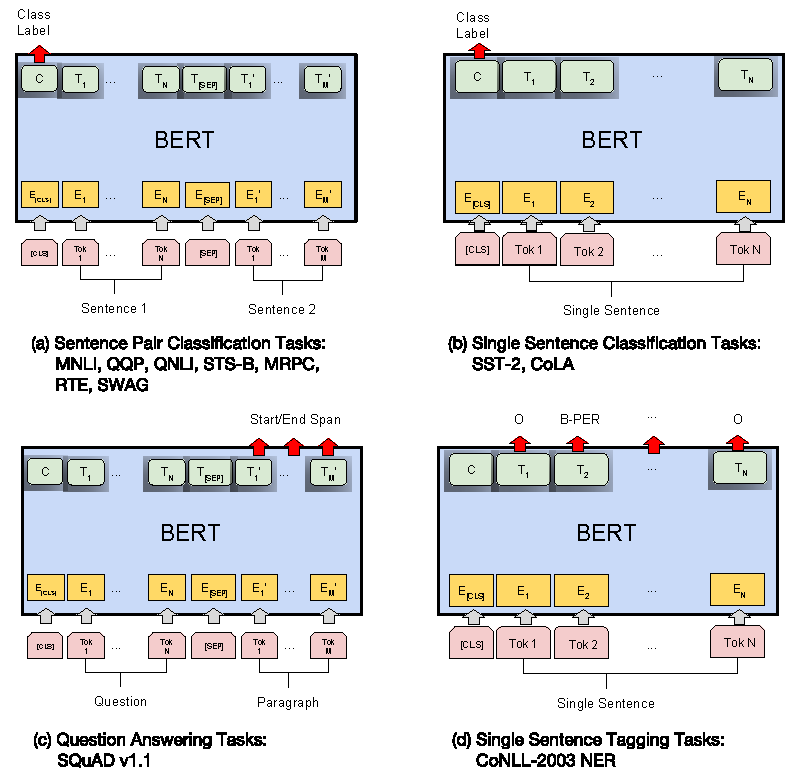
\includegraphics[width=.9\textwidth]{BERTTokenPrediction.png}
	\captionof{figure}{BERT Token Prediction}
	\label{fig:background:berttokenprediction}
\end{center}

Additionally, the model learns specific segment embeddings, which better enables it to separate out and distringuish the two sentences (if both are fed) as input. Finally, since the locations of the tokens in the input sentence matters, and gives termporal information to the model. This is because Transformers do not encode the sequential nature of their inputs \cite{Vaswani} and so this is added as an additional embedding. The three embeddings are summed together, as per the diagram in Figure \ref{fig:background:bertembeddings}.

\begin{center}
	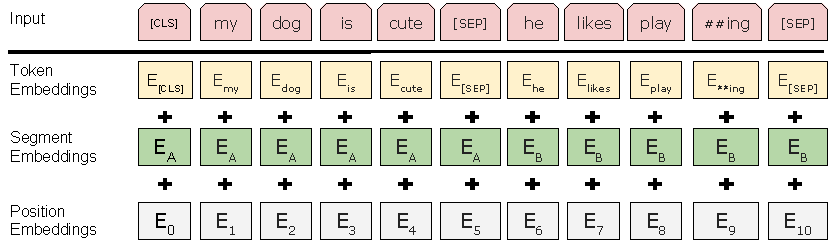
\includegraphics[width=\textwidth]{BERTEmbeddings.pdf}
	\captionof{figure}{BERT Embeddings. In addition to the learned token embeddings, there are segment embeddings (as to whether or not we are in the first sentence or second sentence) and positional embeddings \cite{Vaswani} that help indicate the relative positioning of tokens in the sentence.}
	\label{fig:background:bertembeddings}
\end{center}

\subsubsection{Ablation Study}
The original BERT ablation study looked at 3 model variants:
\begin{enumerate}
	\itemsep0em 
	\item A model with a MLM but without the Next Sentence Prediction (NSP) task
	\item A unidirectional left-to-right LM without NSP
	\item Model above + biLSTM (randomly initialised) thereby ``strengthening" the above model
\end{enumerate}
They showed (Table 5 in \cite{Devlin2018}) that including the NSP task improved the model across all tasks, with major improvements, as expected, on the QNLI task (Question Natural Language Inference, a subtask of the Stanford Question Answering dataset). Additionally, they found that the bidirectional model outperformed the unidirectional one.

While subsequent studies (RoBERTa \cite{Liu2019}, XLNet \cite{Yang2019}, ``Fair XLNet" \cite{XLNetTeam2019}) have agreed with the latter claim, they both disagree with the former, instead finding that next sentence prediction as an auxilliary pretraining task \textit{harms model performance}, including on Question Answering and NLI datasets such as SQuAD and MNLI as well as Sentiment tasks (SST-2 - See Section \ref{section:background:sst2}). Additionally, in the ``Fair XLNet" study, they report different best performing BERT models, claiming that the BERT model trained without the NSP task does perform better than the one trained jointly with it \cite{XLNetTeam2019}. This juxtaposition is explored and tested further in our experimental setup in Section \ref{section:experiments:nlipretrainingimportance}.

\subsubsection{Recreating the NLP Pipeline}
In Section \ref{section:intro:history}, we introduced the NLP pipeline, a notional idea that smaller subtasks are required as ``building blocks" of language understanding, and that any model capable of understanding such downstream language tasks must, in some sense, be able to reconstruct this pipeline. Recently, an interesting paper \cite{Tenney2019} conducted by researchers at Google remarked that certain liguistic information was captured in various layers of the network. By introducing a technique they call ``edge probling" they conclude that different layers of the BERT network can resolve syntactic and semantic structure within a sentence, indicating that the model has some explainability and parallels to human cognition in terms of how it understands language. This makes BERT a prime Language Model for our downstream tasks, since it gives us confidence that this model is able to utilise these subtasks for more important tasks of interest.

\begin{center}
	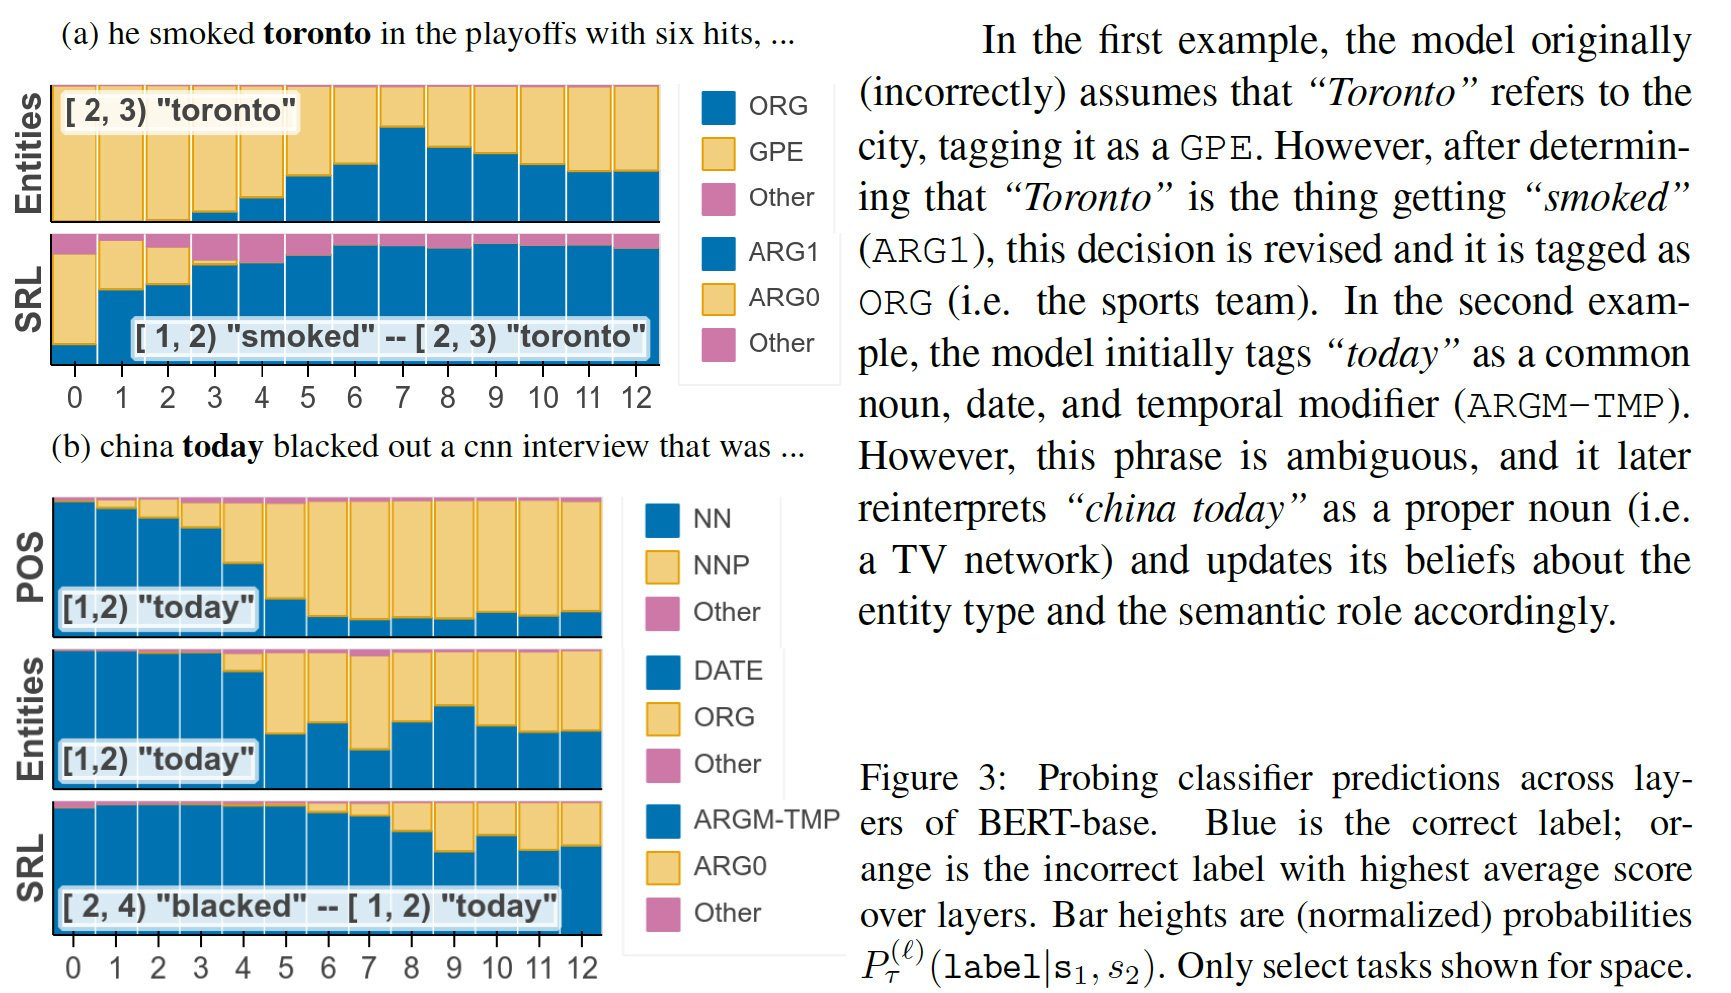
\includegraphics[width=\textwidth]{BERTNLPPipeline.jpg}
	\captionof{figure}{BERT correcting its predictions along the model depth layers, taken from \cite{Tenney2019}}
\end{center}

\subsection{XLNet} \label{section:background:xlnet}
\subsubsection{Autoregressive vs Autoencoding Language Modelling: BERT vs XLNet}
The formulation described in Section \ref{section:background:problemsetup} is referred to as the autoregressive (AR) model. It intends to factorise the likelihood of an input sequence $\mathbf{x} = (w_1, w_2, \dots, w_n)$ into a forward product, or a backward product:
\begin{align*}
\text{Forward Product:} \ & \ \P(\mathbf{x}) = \prod \limits_{t=1}^{T} \P(w_t | \{w_{>t}\}) \\
\text{Backward Product:} \ & \ \P(\mathbf{x}) = \prod \limits_{t=1}^{T} \P(w_t | \{w_{<t}\}) 
\end{align*}
A parametric model (e.g. a neural network) is trained to model each conditional distribution. Since an AR language model is only trained to encode a unidirectional context (either forward or backward), it is not effective at modeling deep bidirectional contexts which we've seen is important for downstream tasks.

As explained in Section \ref{section:background:bert}, BERT gets around this problem by instead using an autoencoding (AE) model; the pretraining does not perform explicit density estimation but instead aims to reconstruct the original data from corrupted input (the \texttt{[MASK]} tokens in BERT). As we've discussed, these artificial \texttt{[MASK]} symbols used by BERT during pretraining are absent from real data at finetuning time, resulting in a pretrain-finetune discrepancy. Furthermore, since the predicted tokens are masked in the input, BERT is not able to model the joint probability using the product rule as in AR language modeling. In other words, BERT assumes the predicted tokens are independent of each other given the unmasked tokens, which is oversimplified as high-order, long-range dependency is prevalent in natural language \cite{Dai2019}.

\subsubsection{Permutation Language Modelling - An alternative pretraining objective}
As a consequence, the authors of XLNet propose a generalized autoregressive method that leverages the best of both AR and AE language modeling and while avoiding their limitations, namely:
\begin{itemize}
	\item Introducing a novel pretraining procedure: fixing either a forward or backward product factorisation but maximise the expected likelihood over \textit{all possible permutations of the factorisation order}. This permutation procedure enables the model to capture bidirectional context since left and right tokens could feasibly appear ``ahead" of the current tokens in the unidirectional model.
	\item As a generalized AR language model, XLNet does not suffer from the pretrain-finetune discrepancy that BERT is subject to. Meanwhile, the autoregressive objective also provides a natural way to use the product rule for factorizing the joint probability of the predicted tokens, eliminating the independence assumption made in BERT.
\end{itemize}
This latter point is important, and the example given in the paper demonstrates the key difference: consider a concrete example [New, York, is, a, city]. Suppose both BERT and XLNet select the two tokens [New, York] as the prediction targets and maximize $\log p(\text{New York} | \text{is a city})$. Also suppose that XLNet samples the factorization order [is, a, city, New, York]. In this case, BERT and XLNet respectively reduce to the following objectives:
\begin{align*}
\mathcal{J}_{\text{BERT}} = \log p(\text{New} | \text{is a city}) + \log p(\text{York} | \text{is a city}) \\
\mathcal{J}_{\text{XLNet}} = \log p(\text{New} | \text{is a city}) + \log p(\text{York} | \text{ {\color{blue} New}, is a city})
\end{align*}
Thus, XLNet is able to capture the dependency between the pair (New, York) which is omitted by BERT, and this leads to a much more effective training signal since XLNet will always be able to capture denser dependency links given this permutation structure and objective.

\subsubsection{Ablation Study}
To investigate the efficacy of the alternative permutation language modelling pretraining objective, as well as design choices such as (importantly to this thesis) the inclusion of the next sentence prediction task, the authors include a comparison of 6 XLNet model variants compared to the original BERT-Base implementation \cite{Devlin2018}. For fair comparison, all models are based on a 12-layer architecture with the same model hyper-parameters as BERT-Base and are trained on only Wikipedia and the BooksCorpus data. They find that the various base models of XLNet outperform BERT on a wide range of tasks, 20 NLP tasks in total. It achieved a 2 point improvement over BERT on all of the GLUE tasks, achieving a combined score of 88.4 to BERT's 80.5 (although RoBERTa \cite{Liu2019} achieved a score of 88.5, showing that BERT can be robustly optimised to match XLNets performance). In terms of relevance for this thesis, it achieves SOTA performance on the SST-2 dataset for Sentiment Analysis (cf. Section \ref{section:background:sst2}) with an accuracy score of 96.8\%, beating BERT's 94.9\%.

Interestingly, the authors note that the inclusion of the next sentence prediction task discussed by the BERT authors harms the model performance across a wide variety of datasets including SST-2 and, more interestingly, MNLI and SQuAD (since, as discussed in Section \ref{section:background:bert}, intuitively we would expect NLI/QA downstream tasks to benefit from NLI pretraining task knowledge), but not RACE (a more challenging reading comprehension task than SQuAD). This feels like an important juxtaposition that is not thoroughly investigated by the authors, and a more rigorous analysis of the next sentence prediction task on NLI and QA downstream tasks should be included, to understand better whether this multitask pretraining objective is a useful feature. Nonetheless, the authors conclude that it is unhelpful, and so omit this auxilliary pretraining objective when training the larger XLNet-Large model. The released set of weights for XLNet-Base do not include this next sentence prediction task, and this is important for a key research question that we investigate in Section \ref{section:experiments:nlipretrainingimportance}.

\subsubsection{Comparisons with BERT}
Upon release of the XLNet paper, the scientific community felt it was unfair to draw direct comparisons between BERT and XLNet, since XLNet used around 10 times more data compared to BERT. Subsequently, the authors followed up the paper with an addendum in the form of a blog post \cite{XLNetTeam2019} where they ensured that almost every possible hyperparameter was the same for both BERT and XLNet as well as pretraining on exactly the same data. 

The study trains 3 separate BERT models, the first being the original one released by the authors, the second being the original model with whole word masking as released by the authors and the third being BERT without the Next Sentence Prediction (NSP) pretraining task since they found the NSP task to harm performance. Despite the Ablation Study in BERT explicitly finding that this task helped in BERT-Base, the XLNet authors report that when training BERT-Large, the best of three variants was often model 2 (10/13 metrics), but occasionally model 3 (3/13 metrics), and never model 1 (0/13 metrics).

They report that even taking the best of these three models, XLNet strictly outperforms BERT across the board on 13 metrics across 11 tasks, albeit by smaller margins than before when it used 10x more data, thus concluding that this model is strictly better than BERT. Recently, however, RoBERTa \cite{Liu2019} ensured the BERT pretraining procedure, and thus the AE approach, was much more robust leading to equal or better performance than XLNet almost unilaterally. These transformer architectures, the interplay between pretraining procedures and downstream fine tuning performance and the relationship between larger and smaller models is not yet well understood by the academic community.

\subsection{Casing in Language Models} \label{section:background:casing}
Language models use a tokenizer to preprocess the input words. Both XLNet and BERT use a type of sentence piece tokenisation methodology to split up words into subpieces that are fed in as tokens. There are typically two settings for this, either capitalisation is preserved (\texttt{cased}) or all the inputs are preprocessed into lower case (\texttt{uncased}).

The BERT models release both \texttt{cased} and \texttt{uncased} versions, with vocabulary sizes of 28,996 and 30522 respectively. The lesser vocabulary size in the cased version, as well as the fact that there are often two sets of the same wordpiece token (one with capitalisation, one without) means that the BERT-\texttt{cased} version tends to have worse learned word representations compared to BERT-\texttt{uncased}. The XLNet models are \texttt{cased} by default. Furthermore, both XLNet and BERT have ``base" versions with fewer parameters, and ``large" versions with more parameters.

Typically, researchers use \texttt{bert-base-uncased} in their research since it has fewer parameters and better learned word representations. Since the XLNet models are so new, not much research has been conducted using them at the time of writing this thesis.

\section{Sentiment Analysis}
Sentiment Analysis is an important downstream task for language modelling. Indeed, one such benchmark dataset for the evaluation of language models is GLUE \cite{Wang2018}, a collection of 9 natural language understanding tasks,  of which the SST-2 (see Section \ref{section:background:sst2})  dataset is a subtask. Often, we fine tune these aforementioned language models on these tasks and, after a hyperparameter search or combination with ensemble models (using multitask learning, as discussed in \ref{section:background:multitasklearningforLMs}), achieve higher metrics scores than custom built models trained from scratch.

A more profound demonstration of sentiment's latent utility in text understanding was a paper \cite{Radford2017} which found that when given sufficient amounts of capacity, training data, and compute time, the representations learned by generative models training to generate customer reviews included disentangled features corresponding to high-level concepts, specifically they found a single unit which performs sentiment analysis. They termed this the ``Unsupervised Sentiment Neuron". These representations, learned in an unsupervised manner, achieved state of the art on the binary subset of the Stanford Sentiment Treebank (SST-2, as discussed in Section \ref{section:background:sst2}).

Sentiment Analysis has often been viewed as a human aspect due to the complex contextual and semantic factors involved, but this makes it an interesting and difficult problem for NLP models that are interesting in the academic sense, but also applicable in the commercial setting (cf. Appendix \ref{appendix:streetbees}). In this section, we outline the key Sentiment Analysis tasks that we will focus on in this thesis.

\subsection{SST-2} \label{section:background:sst2}
The Stanford Sentiment Treebank (SST) is a binary (2 class) or fine grained (5 class) single-sentence classification task consisting of sentences extracted from movie reviews with human annotations of their sentiment \cite{Socher}. It is a popular task on which to test Sentiment Analysis performance, and is included as part of the GLUE tasks.

The aforementioned ``Unsupervised Sentiment Neuron" LSTM model achieved an accuracy of 91.8 on the Binary SST-2 dataset. With the advent of fine tuning language models, we achieved much better accuracy scores than these custom built models. BERT achieved a score of 94.9, an impressive absolute increase of 3\%, further justifying the capabilities of a pretrained language model, and XLNet achieved the (current SOTA) accuracy of 96.8\%, utilising an ensemble model of the larger parameter version of XLNet. RoBERTa, without any ensemble methodologies, achieved 96.7\% - leading to the conclusion that these language models are very similar in terms of sentiment classification (if not undertrained as in the initial version of BERT - discussed in Section \ref{section:background:bert}).

\subsection{SemEval 2014 - ABSA} \label{section:background:semeval}
Aspect-Based Sentiment Analysis (ABSA) aims to identify fine grained opinion polarity towards a specific aspect, and is a more challenging variant of sentiment analysis. It is a vital task from many standpoints, since it provides a more nuanced insight into subparts of a sentence on ``aspects of interest". In particular this makes it academically challenging, since a model would have to account for this, as well as commercially useful. There are many different variants of this task, as outline in Table \ref{table:background:absasubtasks}
\begin{center}
	\begin{tikzpicture}
	% the matrix entries
	\matrix (mat) [table]
	{
		\textbf{Variants} & \textbf{Description} \\
		\textit{Aspect term extraction}& Given a set of sentences with pre-identified entities, identify the distinct aspect terms present in the sentence \\
		\textit{Aspect term polarity} & given a set of aspect terms within a sentence, determine whether the polarity of each aspect term \\
		\raisebox{-5mm}{\shortstack{\textit{Aspect}\\ \textit{Category Detection}}} & given a predefined set of aspect categories (e.g., price, food), identify the aspect categories discussed in a given sentence \\
		\raisebox{-5mm}{\shortstack{\textit{Aspect}\\ \textit{Category Polarity}}} & given a set of pre-identified aspect categories, determine the polarity of each aspect category if it exists in the input sentence \\
	};
	\end{tikzpicture}
	\captionof{table}{Subtasks and variants of ABSA. Typically, the polarity categories are \{\texttt{positive, negative, neutral, conflict}\} where conflict denotes both positive and negative sentiment being expressed simultaneously} \label{table:background:absasubtasks}
\end{center}	

Task 4 of the SemEval-2014 Workshop focuses on this task, for which there are 4 subtasks (relating to the variants described Table \ref{table:background:absasubtasks}).  We focus specifically on Subtask 4 i.e. given a set of known, fixed aspects $\mathcal{A}$, and a set of fixed sentiment criterion classes $\mathcal{C}$: for each sentence $x$ in the dataset, of which aspects $\mathcal{A}' \subseteq \mathcal{A}$ appear, classify each $a_x \in \mathcal{A}'$ with one sentiment class $c(a_x) \in \mathcal{C}$. We focus on the restaurant dataset\footnote{motivated by tits similarity to the type of data the company works on - see Appendix \ref{appendix:streetbees}} which has:
\begin{gather*}
\mathcal{A} = \{ \texttt{food, service, price, ambience, anecdotes/miscellaneous}\} \\
\mathcal{C} = \{ \texttt{positive, negative, neutral, conflict, none}\}
\end{gather*}

At the time the challenge was released (2014, prior to all advanced language modelling discussions in Section \ref{section:background:LMs}), the champion model was using crafted features based on specifically constructed lexicon features from various datasets, Part Of Speech (PoS) and Named Entity Recognition (NER) tagging (discussed in Section \ref{section:methodology:datasets}) and word and character level $n$-grams concatenated into a feature vector and put through a SVM model \cite{Kiritchenko2014}. This model was specifically domain adapted towards the restaurant task, and as such does not represent the scalability and generalisation capability to other tasks of language models such as BERT and XLNet. Nonetheless, this model outperformed all other approaches, achieving an accuracy of 82.93\% which is impressive given the task difficulty.

Recently, BERT, as discussed in Section \ref{section:background:bert}, was applied to this task but did not yield big performance increases over the traditional, custom built models like the one described above, achieving an accuracy of 83.7\% (an improvement just shy of 1\%) \cite{Sun2019}. However, the same paper proposed a novel auxilliary sentence technique whereby either auxilliary questions or pseudosentences were augmented to the input text and joint classification was performed. There were many variants of this (described in Section \ref{section:background:tabsasentenceconstruction}), but this method pushed the accuracy up to 85.9\% - a 3\% increase on the traditional custom built models.
\subsection{Sentihood - TABSA} \label{section:background:sentihood}
Target-ABSA (TABSA) generalises this notion one stage further: applying ABSA for each target entity $t$. An example from the Sentihood dataset is included in Table \ref{table:background:tabsaexample}

\begin{center}
\begin{tabular}{|c|c|c|}
	\hline
	Target & Aspect & Sentiment \\
	\hline
	{\color{black} LOCATION1} & {\color{purple} general} & {\color{green} Positive} \\
	{\color{black} LOCATION1} & {\color{cyan} price} & {\color{gray} None} \\
	{\color{black} LOCATION1} & {\color{orange} safety} & {\color{gray} None} \\
	{\color{black} LOCATION1} & {\color{pink} transit-location} & {\color{gray} None} \\
	\hline \hline
	{\color{black} LOCATION2} & {\color{purple} general} & {\color{gray} None} \\
	{\color{black} LOCATION2} & {\color{cyan} price} & {\color{red} Negative} \\
	{\color{black} LOCATION2} & {\color{orange} safety} & {\color{gray} None} \\
	{\color{black} LOCATION2} & {\color{pink} transit-location} & {\color{green} Positive} \\
	\hline
\end{tabular}
\captionof{table}{TABSA Example: {\color{black} LOCATION2} is in central London, and thus extremely expensive, whilst {\color{black} LOCATION1} is often considered the coolest area of London.} \label{table:background:tabsaexample}
\end{center}

\subsection{(T)ABSA and LMs: Auxilliary Sentence Construction Method} \label{section:background:tabsasentenceconstruction}
As eluded to in Sections \ref{section:background:semeval} and \ref{section:background:sentihood}, the current SOTA method developed this year for solving (T)ABSA style problems includes a novel (pseudo)sentence augmentation method, which researchers show strictly outperforms \textit{just} applying the language model to the problem in the multiclass classification setting \cite{Sun2019}. In this section, we detail the method, as it is integral to the thesis, and critically analyse the paper.
\begin{center}
	\resizebox{\textwidth}{!}{%
	\begin{tabular}{|c|c|c|}
		\hline
		NLI-\textbf{B} & QA-\textbf{B} & Label \\
		\hline \hline
		\textit{{\color{black} location - 1} - {\color{purple} general} - {\color{green} positive}} & \textit{is the polarity of the aspect {\color{purple} general} of {\color{black} location - 1} {\color{green} positive}?} & 1 \\
		\textit{{\color{black} location - 1} - {\color{purple} general} - {\color{red} negative}} & \textit{is the polarity of the aspect {\color{purple} general} of {\color{black} location - 1} {\color{red} negative}?} & 0 \\
		\textit{{\color{black} location - 1} - {\color{purple} general} - {\color{gray} none}} & \textit{is the polarity of the aspect {\color{purple} general} of {\color{black} location - 1} {\color{gray} none}?} & 0 \\
		\hline \hline
		\textit{{\color{black} location - 1} - {\color{cyan} price} - {\color{green} positive}} & \textit{is the polarity of the aspect {\color{cyan} price} of {\color{black} location - 1} {\color{green} positive}?} & 0 \\
		\textit{{\color{black} location - 1} - {\color{cyan} price} - {\color{red} negative}} & \textit{is the polarity of the aspect {\color{cyan} price} of {\color{black} location - 1} {\color{red} negative}?} & 0 \\
		\textit{{\color{black} location - 1} - {\color{cyan} price} - {\color{gray} none}} & \textit{is the polarity of the aspect {\color{cyan} price} of {\color{black} location - 1} {\color{gray} none}?} & 1 \\
		\hline \hline
		\textit{{\color{black} location - 1} - {\color{orange} safety} - {\color{green} positive}} & \textit{is the polarity of the aspect {\color{orange} safety} of {\color{black} location - 1} {\color{green} positive}?} & 0 \\
		\textit{{\color{black} location - 1} - {\color{orange} safety} - {\color{red} negative}} & \textit{is the polarity of the aspect {\color{orange} safety} of {\color{black} location - 1} {\color{red} negative}?} & 0 \\
		\textit{{\color{black} location - 1} - {\color{orange} safety} - {\color{gray} none}} & \textit{is the polarity of the aspect {\color{orange} safety} of {\color{black} location - 1} {\color{gray} none}?} & 1 \\
		\hline \hline
		\textit{{\color{black} location - 1} - {\color{pink} transit-location} - {\color{green} positive}} & \textit{is the polarity of the aspect {\color{pink} transit-location} of {\color{black} location - 1} {\color{green} positive}?} & 0 \\
		\textit{{\color{black} location - 1} - {\color{pink} transit-location} - {\color{red} negative}} & \textit{is the polarity of the aspect {\color{pink} transit-location} of {\color{black} location - 1} {\color{red} negative}?} & 0 \\
		\textit{{\color{black} location - 1} - {\color{pink} transit-location} - {\color{gray} none}} & \textit{is the polarity of the aspect {\color{pink} transit-location} of {\color{black} location - 1} {\color{gray} none}?} & 1 \\
		\hline \hline
		\textit{{\color{black} location - 2} - {\color{purple} general} - {\color{green} positive}} & \textit{is the polarity of the aspect {\color{purple} general} of {\color{black} location - 2} {\color{green} positive}?} & 0 \\
		\textit{{\color{black} location - 2} - {\color{purple} general} - {\color{red} negative}} & \textit{is the polarity of the aspect {\color{purple} general} of {\color{black} location - 2} {\color{red} negative}?} & 0 \\
		\textit{{\color{black} location - 2} - {\color{purple} general} - {\color{gray} none}} & \textit{is the polarity of the aspect {\color{purple} general} of {\color{black} location - 2} {\color{gray} none}?} & 1 \\
		\hline \hline
		\textit{{\color{black} location - 2} - {\color{cyan} price} - {\color{green} positive}} & \textit{is the polarity of the aspect {\color{cyan} price} of {\color{black} location - 2} {\color{green} positive}?} & 0 \\
		\textit{{\color{black} location - 2} - {\color{cyan} price} - {\color{red} negative}} & \textit{is the polarity of the aspect {\color{cyan} price} of {\color{black} location - 2} {\color{red} negative}?} & 1 \\
		\textit{{\color{black} location - 2} - {\color{cyan} price} - {\color{gray} none}} & \textit{is the polarity of the aspect {\color{cyan} price} of {\color{black} location - 2} {\color{gray} none}?} & 0 \\
		\hline \hline
		\textit{{\color{black} location - 2} - {\color{orange} safety} - {\color{green} positive}} & \textit{is the polarity of the aspect {\color{orange} safety} of {\color{black} location - 2} {\color{green} positive}?} & 0 \\
		\textit{{\color{black} location - 2} - {\color{orange} safety} - {\color{red} negative}} & \textit{is the polarity of the aspect {\color{orange} safety} of {\color{black} location - 2} {\color{red} negative}?} & 0 \\
		\textit{{\color{black} location - 2} - {\color{orange} safety} - {\color{gray} none}} & \textit{is the polarity of the aspect {\color{orange} safety} of {\color{black} location - 2} {\color{gray} none}?} & 1 \\
		\hline \hline
		\textit{{\color{black} location - 2} - {\color{pink} transit-location} - {\color{green} positive}} & \textit{is the polarity of the aspect {\color{pink} transit-location} of {\color{black} location - 2} {\color{green} positive}?} & 1 \\
		\textit{{\color{black} location - 2} - {\color{pink} transit-location} - {\color{red} negative}} & \textit{is the polarity of the aspect {\color{pink} transit-location} of {\color{black} location - 2} {\color{red} negative}?} & 0 \\
		\textit{{\color{black} location - 2} - {\color{pink} transit-location} - {\color{gray} none}} & \textit{is the polarity of the aspect {\color{pink} transit-location} of {\color{black} location - 2} {\color{gray} none}?} & 0 \\
		\hline
	\end{tabular}}
	\captionof{table}{\textbf{B}inary Auxilliary Sentence Construction Method for example in Table \ref{table:background:tabsaexample}} \label{table:background:tabsasentencesB}
	\resizebox{\textwidth}{!}{%
	\begin{tabular}{|c|c|c|}
		\hline
		NLI-\textbf{M} & QA-\textbf{M} & Label \\
		\hline
		\textit{{\color{black} location - 1} - {\color{purple} general}} & \textit{what do you think of the {\color{purple} general} of {\color{black} location - 1}?} & {\color{green} Positive} \\
		\textit{{\color{black} location - 1} - {\color{cyan} price}} & \textit{what do you think of the {\color{cyan} price} of {\color{black} location - 1}?} & {\color{gray} None} \\
		\textit{{\color{black} location - 1} - {\color{orange} safety}} & \textit{what do you think of the {\color{orange} safety} of {\color{black} location - 1}?} & {\color{gray} None} \\
		\textit{{\color{black} location - 1} - {\color{pink} transit - location}} & \textit{what do you think of the {\color{pink} transit - location} of {\color{black} location - 1}?} & {\color{gray} None} \\
		\hline \hline
		\textit{{\color{black} location - 2} - {\color{purple} general}} & \textit{what do you think of the {\color{purple} general} of {\color{black} location - 2}?} & {\color{gray} None} \\
		\textit{{\color{black} location - 2} - {\color{cyan} price}} & \textit{what do you think of the {\color{cyan} price} of {\color{black} location - 2}?} & {\color{red} Negative} \\
		\textit{{\color{black} location - 2} - {\color{orange} safety}} & \textit{what do you think of the {\color{orange} safety} of {\color{black} location - 2}?} & {\color{gray} None} \\
		\textit{{\color{black} location - 2} - {\color{pink} transit - location}} & \textit{what do you think of the {\color{pink} transit - location} of {\color{black} location - 2}?} & {\color{green} Positive} \\
		\hline
	\end{tabular}}
	\captionof{table}{\textbf{M}ultickass Auxilliary Sentence Construction Method for example in Table \ref{table:background:tabsaexample}} \label{table:background:tabsasentencesM}
\end{center}

The authors suggest the following sentence augmentation procedures outlined in Tables \ref{table:background:tabsasentencesB} and \ref{table:background:tabsasentencesM} that augment the input sentence with either a question or a pseudosentence, and have the classification be either binary or multiclass. They instantiate the pretrained BERT \cite{Devlin2018} model, and fine tune on this modified dataset to show that this procedure strictly outperforms the base case of just performing multiclass classification on the input sentences alone, conjecturing that the performance improvements from this technique leverage the models ability to perform well at NLI (and QA) tasks due to the next sentence prediction pretraining objective (discussed in Section \ref{section:background:bert}). The 4 different models achieve different top metrics on the Sentihood task, but they find on the SemEval task 4, subtask 4 (as described in Section \ref{section:background:semeval}) that the QA-\textbf{B} model achieves the highest accuracies on the SemEval dataset, as well as the highest $F_1$ score for aspects and AUC score for sentiments on the Sentihood data. We will refer to this as the TABSA ``explosion" method, as detailed in the next section.

\subsection{Analysis of the TABSA Explosion Method}
Since this method converts the (target and) aspect information into an auxilliary sentence, this is equivalent to exponentially expanding the corpus. We refer to this process as ``exploding the dataset". For a given unique input text, if there are $n_t$ target entities and $n_a$ aspects, then the datapoint is exploded into $n_t \cdot n_a$ new datapoints, where the secondary sentence that is augmented to the model determined uniqueness of the sentence pairs. On the one hand, this creates a much \textit{sparser} dataset, since many of the labels are of the null class (either `None' or 0 in the multiclass and binary cases respectively). This would almost certainly harm training if the model were learning from scratch. However, since we are initialising the language model with pretrained weights, the authors conjecture that, since BERT in particular has been trained with a next sentence prediction pretraining objective simultaneously to its Cloze task, the model is able to learn from this data since it already has some prior knowledge about NLI and QA tasks from which it can transfer learn.

The binary explosion is also interesting in the setting where the aspects are nonunique, i.e. in multilabelled data. If the aspects were instead just categories themselves, such as emotions\footnote{This is an example we will return to when looking at the industry specific dataset, cf Section \ref{section:data:streetbees}} then it could be that a person is feeling multiple emotions simultaneously. This binary approach, since the final layer is a sigmoid, will give us the probabilities of each emotion. Then, multilabel categorisation can be performed if this probability is over a certain threshold (say 0.5).

However, one drawback of this method is the computational considerations when expanding the dataset in this way. The multiclass problem means the instantiation of more parameters for each class head, but the binary explosion means much more forward passes through the model and thus a longer training time overall so there is a tradeoff.


\section{Multitask learning} \label{section:background:multitask}
In Machine Learning, we often care about optimising a particular metric of interest. In order to do this, we generally train a single model or possibly an ensemble of models that all individually try to optimise this metric to perform our desired task. We then finetune and tweak these models until their performance no longer increases. However, this might be a myopic framing of the problem; while we can generally achieve acceptable performance this way we are ignoring information that might help us do even better on the metric we care about. Specifically, this information comes from the training signals of related tasks. By sharing representations between related tasks, we can enable our model to generalise better on our original task. This is precisely the multitask learning paradigm.

One form of Multitask learning is so called \textit{continual learning} or \textit{sequential transfer learning} \cite{Parisi2018, RuderThesis} which aims to train the model with several tasks in sequence so that it remembers the previously learned tasks when learning the new ones. This method is inspired by the human learning process, since we are capable of continuously accumulating the information acquired by study or experience to efficiently develop new skills. With continual learning, the model should be able to performs well on new tasks due to the knowledge acquired during previous training. We could define transfer learning as a means to extract knowledge from a source setting and apply it to a different target setting, as demonstrated in Figure \ref{fig:background:transferlearning}.
\begin{center}
	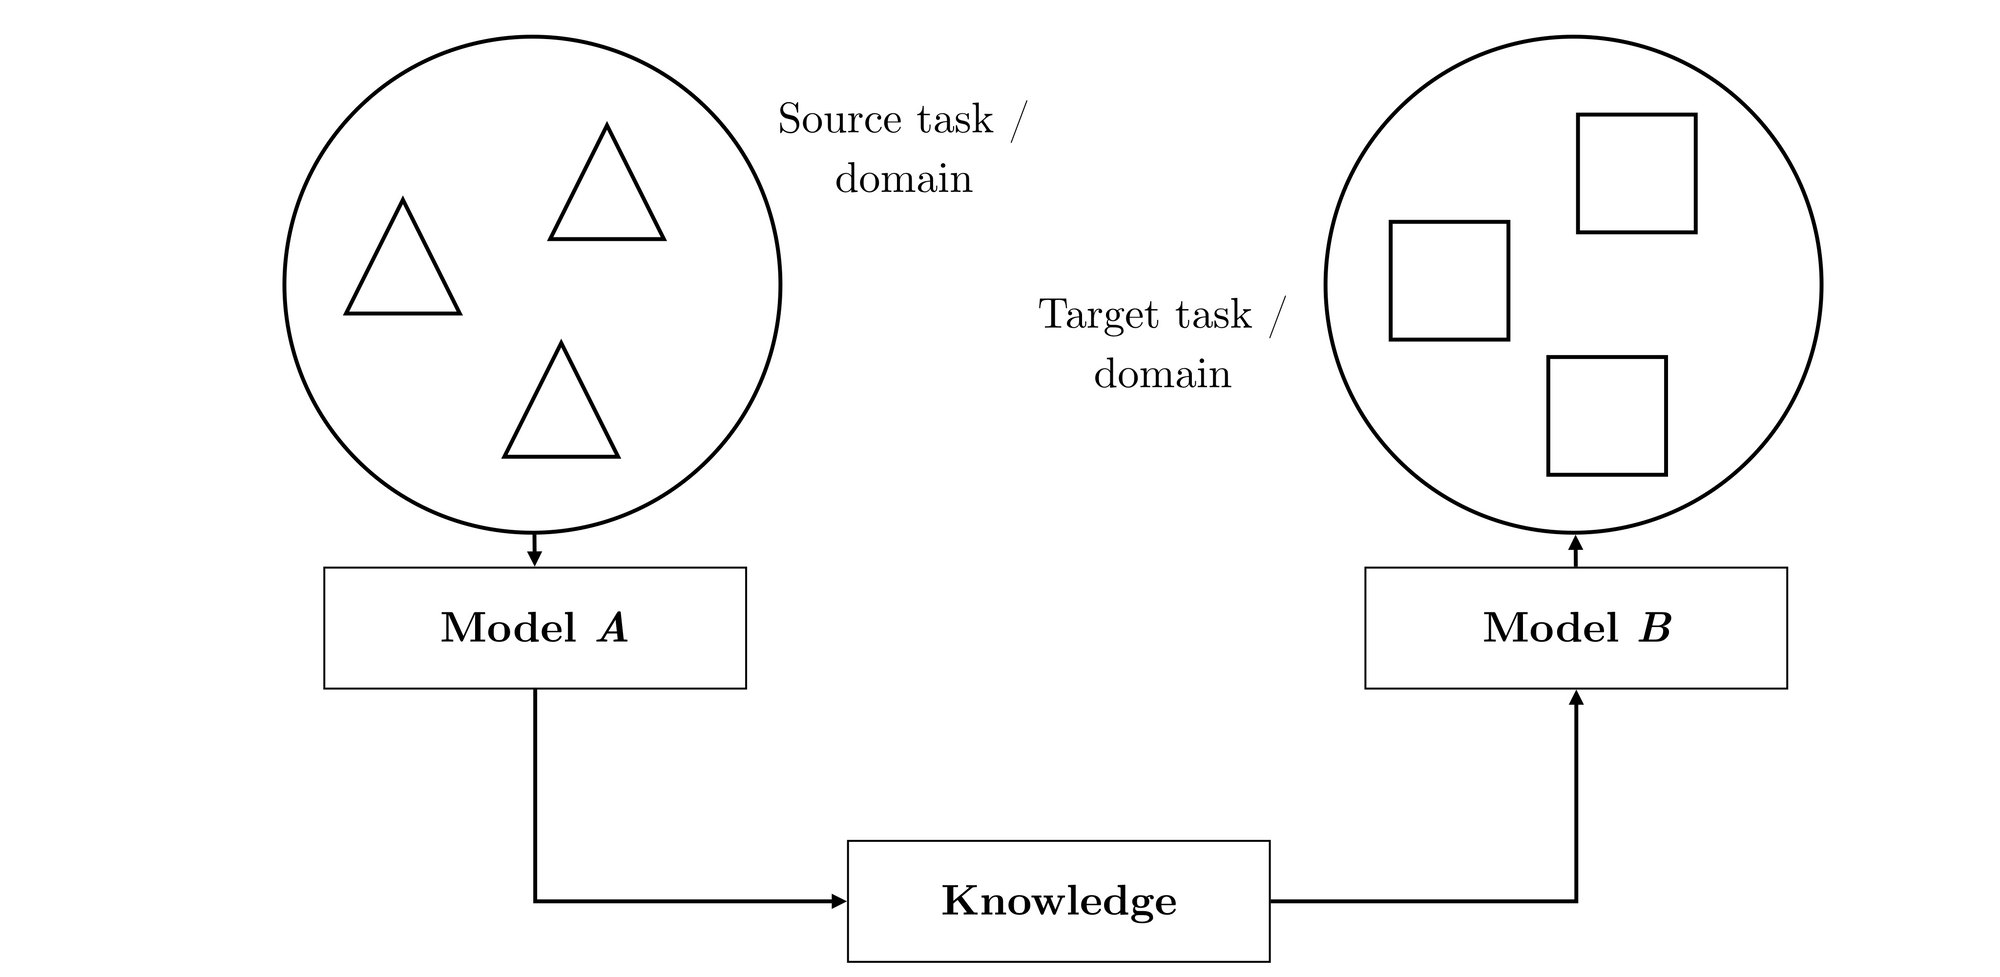
\includegraphics[width=\textwidth]{transfer_learning_scenario.png}
	\captionof{figure}{Transfer Learning Illustration}
	\label{fig:background:transferlearning}
\end{center}

Instead of training sequentially, we could train simultaneously (or ``jointly"). Our hope is that during this joint training and optimisation of many different loss signals we will get improved generalization on our main task by leveraging the domain-specific information contained in the training signals of related tasks. We could motivate multitask learning biologically: from a pedagogical perspective, we often learn tasks first that provide us with the necessary skills to master more complex techniques. We could also motivate it in a statistical and mathematical context by viewing multitask learning as a form of \textit{inductive transfer}. Inductive transfer can help improve a model by introducing an inductive bias, which causes a model to prefer some hypotheses over others. In the case of joint multitask learning, the inductive bias is provided by the auxiliary tasks and thus acts as a form of regularisation since the model learns to prefer hypotheses that explain more than one task.

\subsection{Types of Multitask Learning}
\subsubsection{Hard Parameter Sharing}
\begin{center}
	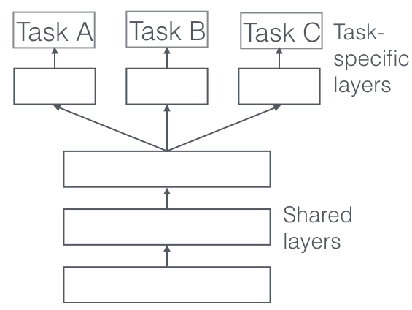
\includegraphics[width=0.5\textwidth]{HardParameterSharing.png}
	\captionof{figure}{Hard Parameter Sharing, with image taken from \cite{Ruder2017}}
	\label{fig:background:hardparametersharing}
\end{center}

One common form of joint multitask learning is hard parameter sharing: we share hidden layers between all tasks, and have task specfic output layers and architectures ``on top" of our hidden layers which filter through to the task loss signal. This is an extremely common form for Language Modelling, and what we focus on in this thesis. The motivation is that a learned Language Model, such as those described in Section \ref{section:background:LMs}, have already in some sense ``learned language" and have a reasonable manifold on which the embeddings lie. Then, in order to perform downstream tasks, we just need simple linear layers which act as projection transformations on this space. This is shown diagramatically in Figure \ref{fig:background:hardparametersharing}

Hard parameter sharing reduces overfitting. This can be seen mathematically \cite{Baxter1997} or intuitively: the more tasks we are learning simultaneously, the more our model has to find a representation that captures all of the tasks and the less is our chance of overfitting on our original task.

\subsubsection{Soft Parameter Sharing} \label{section:background:softparametersharing}
\begin{center}
	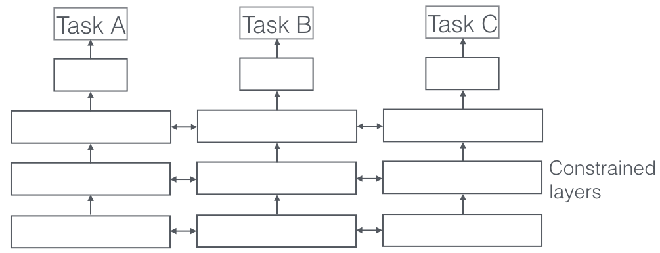
\includegraphics[width=0.5\textwidth]{SoftParameterSharing.png}
	\captionof{figure}{Soft Parameter Sharing, with image taken from \cite{Ruder2017}}
	\label{fig:background:softparametersharing}
\end{center}

Another common method is soft parameter sharing: each task has its own model architecture, but the weights between each layer is ``linked" and regularised in order to encourage these parameters to have ``similar" values. This is shown in Figure \ref{fig:background:softparametersharing}. It is widely recognised that this method is infeasible for language models due to the large number of parameters, and thus duplication/scaling linearly with the number of tasks is computationally intractible.

\subsubsection{Adaption Modules}
A middle ground between the two has been explored, where additional architecture is implemented on top of the pre-existing architecture in an attempt to learn the contributions from each hidden layer and weight them appropriately. The most current SOTA review was Projected Attention Layers (PALs) in a paper titled: BERT and PALs \cite{Stickland2019}. The authors investigated a wide range of these adaption modules, including skip connections and learned layer weighting and propose an alternative attention based architecture (PALs) which use a low-dimensional multihead attention mechanism, based on the idea that it is important to include layers with inductive biases useful for the input domain. 

\subsection{Sampling Tasks} \label{section:background:samplingtasks}
A simple way to train a model on several tasks is to select a batch of training examples from each task, cycling through them in a fixed order. This is often referred to as ``round-robin" sampling, but we will refer to it as ``sequential" sampling (cf. our definitions in Section \ref{section:methodology:taskdistributions}). However, a downside to this strategy is that if each task has a different number of training examples then by the time we have seen every example from a particular task we could have looped through another, smaller tasks dataset many times. This could lead to overfitting on smaller tasks, and undertraining on larger tasks. Potentially we could alleviate this issue by manually tuning regularisation hyper-parameters for each task.
Alternatively we could employ methods where we see more examples from tasks with larger associated datasets. Concretely, we select a batch of examples from task $\tau_i$ with probability $p_{\tau_i}$ at each training step, and set $p_{\tau_i}$ proportional to $m_{\tau_i}$, the number of training examples for task $\tau_i$. This is the approach of the multi-task BiLSTM of the authors in the initial GLUE benchmark paper \cite{Wang2018}, and was used by authors in a Hierarchichal Multitask Approach for learning embeddings from semantic tasks \cite{Sanh2018} . It has the appealing property of selecting each example with the same probability as combining all the tasks and picking examples uniformly (though we train on batches from each task not single examples). This is also the approach used in BERT and PALs \cite{Stickland2019}.

What researchers found by employing these techniques, is that the final metric score does not change too much depending on the sampling schema in this setting; i.e that the sequential sampling mode is sufficient to get good improvements in the multitask learning setting. The main novel approach in this thesis is to redefine the task sampling schemas with a more biologically motivated model. The previous approach can conflate number of examples with ``difficulty of a task", since a task with more examples is sampled more. We find when considering certain datasets that this is not always the case, indeed SST-2 has 67,000 training examples but is considered quite an easy task\footnote{the reader is referred to Table \ref{table:methodology:datasets} for a breakdown of our datasets used in this thesis} and so this is almost certainly a downside of this technique. Instead, we want to employ a more reasonable strategy: sampling proportional to a hierarchichal task structure, leveraging useful subtask properties and sampling our ``main task" more frequently. The details of this methodology are deferred to Sections \ref{section:methodology:taskstructure} and \ref{section:methodology:taskdistributions}.

\subsection{Multitask learning applied to language modelling} \label{section:background:multitasklearningforLMs}
When looking at the leaderboard for the GLUE tasks \cite{Wang2018}, the best performing models on each task are actually ensemble models that are jointly trained on all of, or a subset of, the tasks. However, these tasks that the models are jointly fine tuned on are generally somewhat unrelated and this thesis proposes a different viewpoint regarding ``supporting subtasks" and optimal schemas thereof. For example, In Table 4 of the XLNet Paper \cite{Yang2019}, the authors present results of multiple settings, including single-task and multi-task, as well as single models and ensembles. In the multi-task setting, they jointly train an XLNet on the four largest datasets—MNLI, SST-2, QNLI, and QQP—and finetune the network on each of the other datasets in GLUE. Only single-task training is employed for the four large datasets to achieve the results posted. This decision is somewhat arbritrary, as described earlier.


\subsubsection{ERNIE 2.0}
The authors of ERNIE 2.0 \cite{Sun2019a} propose a way to integrate multitask learning into the pretraining of deep language models. Current pre-training procedures such as the ones in BERT \cite{Devlin2018} and XLNet \cite{Yang2019} described in Sections \ref{section:background:bert} and \ref{section:background:xlnet} usually focus on training the model with several simple tasks to grasp the co-occurrence of words or sentences. However, besides co-occurring, the authors argue that there exists other valuable lexical, syntactic and semantic information in training corpora, such as named entity, semantic closeness and discourse relation that these pretraining protocols do not fully capture. Thus, in order to extract the full lexical, syntactic and semantic information from training corpora, they propose a continual pre-training framework named ERNIE 2.0 which builds and learns incremental pretraining tasks through constant multitask learning. This methodology is outlined in \ref{fig:background:ernie}

\begin{center}
	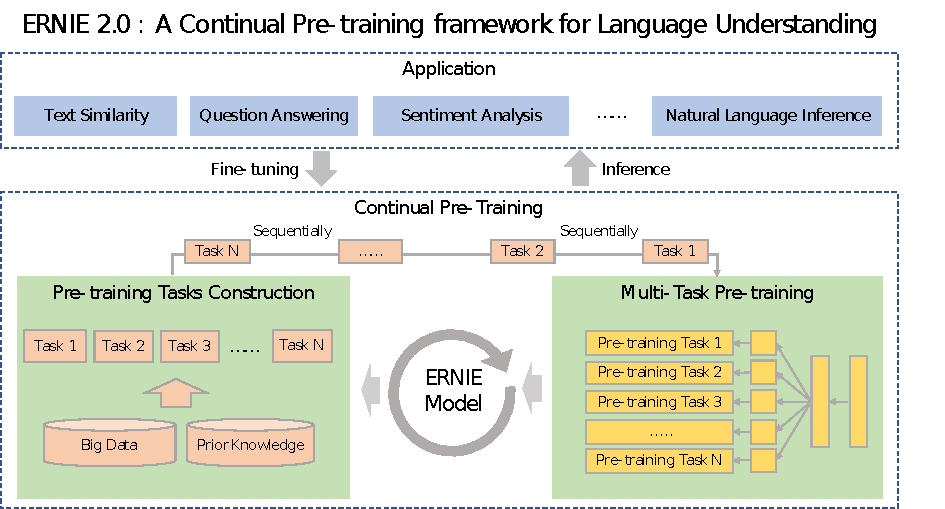
\includegraphics[width=.75\textwidth]{ERNIE2.pdf}
	\captionof{figure}{ERNIE 2.0 Methodology \cite{Sun2019a}}
	\label{fig:background:ernie}
\end{center}

While this paper will focus on Multitask learning as a downstream task, the authors of this recent paper flip this on its head, and realise that multitask learning could instead be used to learn better word embeddings at the pretraining step. This novel idea was originally proposed in the extensions to this thesis prior to the paper being released.

The authors split the pretraining tasks into three categories: ``word-aware" tasks, ``structure-aware" tasks and ``semantic-aware" tasks. The word-aware tasks teach the model to capture the lexical information, the structure-aware tasks teach the model to capture the syntactic information of the corpus and the semantic-aware tasks prioritise the semantic signals. These tasks are represented in Figure \ref{fig:background:ernietaskstructure}, but the reader is referred to the paper \cite{Sun2019a} since the tasks are not that relevant to describe for the purposes of this thesis, but essentially expand on the dual task pretraining framework of BERT \cite{Devlin2018}.

\begin{center}
	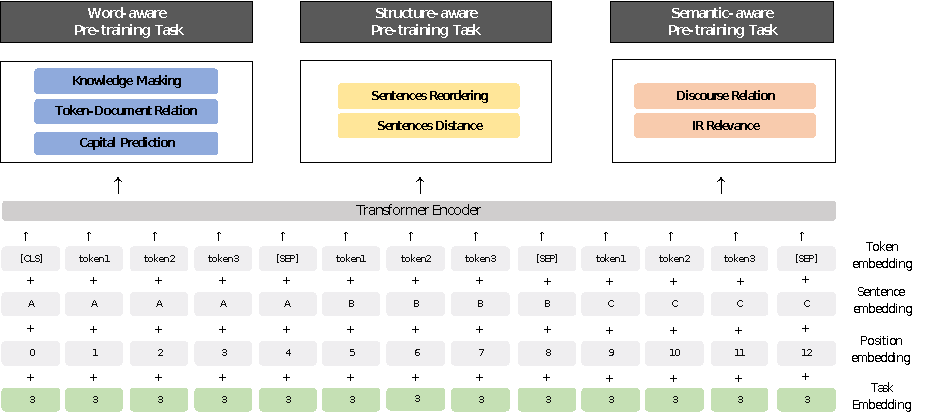
\includegraphics[width=.9\textwidth]{ERNIE2TaskStructure.pdf}
	\captionof{figure}{ERNIE 2.0 Pretraining Task Framework \cite{Sun2019a}}
	\label{fig:background:ernietaskstructure}
\end{center}

\subsection{Multitask learning applied to ABSA}
There hasn't been much work on improving ABSA tasks using multitask learning. We propose to investigate both the classical multitask learning setting of jointly training on tasks, but also generalise this methodology in terms of jointly training via sampling tasks according to a preimposed task importance structure.

\subsection{Multitask learning for Knowledge Graph Construction}
It is clear that from the (T)ABSA methods we can construct the type of Knowledge Graphs (KGs) we motivated at the beginning of the thesis, as per Figure \ref{fig:intro:absa}. Additionally, if combined with NER tasks (or indeed other NLP tasks of interest), this type of framework could also be adapted into multitask multielement learning of the knowledge graph, in terms of the identificiation of entities and then aspect related classification of those entities. 

This knowledge graph could then be used for downstream link prediction of missing elements in the graph. An interesting and novel methodology for this, proposed by researchers at Streetbees and in proceedings for the upcoming EurNLP conference \cite{Garland2019}, proposes converting this knowledge graph into its induced grammar by creating pseudosentences that summarise the original input sentence in terms of key facts (using various weighted walk strategies over subgraphs) and using a language model to end-to-end learn this grammar. Then, link prediction just becomes next token prediction on this vocabulary of entities. However, there are much more standard graph embedding techniques capable of embedding this KG, and optionally performing link prediction \cite{Cai2017}.

\section{Meta Learning} \label{section:background:meta}
Human learning is the benchmark for intelligence, and since humans do not (tend to) learn from thousands or hundreds of thousands of examples, but instead from just a few. We would want our artificial agents to be able to do the same, learning and adapting quickly from only a few examples, and continuing to adapt as more data becomes available. This kind of fast and flexible learning is challenging, since the agent must integrate its prior experience with a small amount of new information, while avoiding overfitting to the new data. In short, we want an algorithm to learn to learn, to be able to learn structured priors from a variety of tasks and be able to apply this prior knowledge effectively on a new task on which it has limited experience of. This is precisely the goal of meta learning.

Suppose we can already solve some set of tasks $\mathcal{T} = \{\tau_1, ..., \tau_n \}$ and we are faced with some new task $\tau^*$. How do we learn it? The transfer learning and multitask learning paradigms state that we could initialise a model with the parameters of some pretrained network, and since this model has learned to solve similar tasks before it might be able to, after a bit of fine tuning, solve our new task. The meta learning framework instead approaches it from a different angle: what if we specifically set up our model training procedure to generalise between tasks? Then, when presented with a new task, since the model has been trying to optimise its generalisation capabilities and learned a set of weights that is ``close" to all of the optimal manifolds for each task \cite{Finn2017}, we still fine tune on our task but its able to generalise to the new task with a limited number of examples since it was explicitly trained to do this, unlike multitask learning.

\subsection{How we learn to learn}
In this thesis we will use a consistent notation for the meta learning terminology, which we outline in this section. Additionally, we will highlight the key changes when going from the traditional learning paradigm to the meta learning one.

In multitask learning, given a set of tasks $\mathcal{T}$, we are training the model to find a set of weights that jointly solves all tasks. In meta learning, given a set of tasks $\mathcal{T}$, we are training our model to learn a set of weights that is able to generalise from any task in $\mathcal{T}$ to any other task in $\mathcal{T}$. This is a more conservative setup and will probably not be able to perform better at each of the individual tasks in $\mathcal{T}$ compared to multitask learning, but it is able to generalise to new tasks much more effectively since that was how the model was trained.

The main difference between meta learning and regular learning is that \textit{datapoints in meta learning are datasets}. In the meta learning paradigm, we aim to improve generalisation onto new datasets (corresponding to new tasks), as opposed to individual datapoints in the regular learning paradigm. This means we shift our training and testing procedure to instead train, validate and test on (small) \textit{datasets}.  We have a support set $\mathcal{S}$ and a query set $\mathcal{Q}$. The support set is a set of meta training datapoints, which are themselves datasets of tasks. Task $\tau_i$ has associated training and testing datasets $\mathcal{D}_\text{train}^{(i)}$ and $\mathcal{D}_\text{test}^{(i)}$. The training and testing datasets will be performing $K$ shot learning, i.e learning to classify from just $K$ examples, and will thus be of size $K$. The support set and query set will be of size \texttt{meta\_train\_batch\_size} and \texttt{meta\_test\_batch\_size}, respectively.

\subsection{MAML}
We ideally want an algorithm for meta learning to be model agnostic, and this is what is proposed by Finn et al. in their Model Agnostic Meta Learning (MAML) algorithm \cite{Finn2017}. As long as the model is trained by (some variant of) Gradient Descent \cite{Ruder}, we can use this algorithm to update the weights of our model in a way that is mathematically consistent with the type of behaviour we motivated in the previous paragraph.

In their approach, the parameters of the model are explicitly trained such that a small number of gradient steps with a small amount of training data from a new task will produce good generalization performance on that task. In order to get this behaviour, we would want the models internal representation to be broadly suitable for many tasks. Their evaluation shows that this algorithm compares favorably to state-of-the-art one-shot learning methods designed specifically for supervised classification, while using fewer parameters, but that it can also be readily applied to regression and reinforcement learning settings.

Algorithm \ref{alg:background:maml} shows the pseudocode for the MAML algorithm, and one can clearly see that it makes no \textit{a priori} assumptions on the model. There are two key components: the inner training step, which uses some setting of the base model parameters to calculate batchwise updates over tasks and the meta training step, which uses these adjusted model parameters to calculate the loss function, and take a gradient descent step in the average loss direction to update our base model parameters ready for the next inner training loop on a new batch of tasks.

\begin{algorithm}
	\caption{Model Agnostic Meta Learning (MAML) \cite{Finn2017}}
		\label{alg:background:maml}
	\begin{algorithmic}[1]
		\Require{p($\mathcal{T}$) - distribution over tasks}
		\Require{$\alpha, \beta$ - inner and outer learning rates/step sizes}
		\Require{Model $f_\theta$}
		\State {Randomly Initialise $\theta$, the model weights}
		\While{not done}
			\State {Sample batch of tasks $\mathcal{B} = \{\tau_i\} \sim p(\mathcal{T})$}
			\For{$\tau_i$ in $\mathcal{B}$}
				\State{Evaluate $\nabla_\theta \mathcal{L}_{\tau_i}(f_\theta)$ with respect to $K$ examples} \Comment{$K$ shot learning}
				\State {// \textit{Compute adapted parameters with gradient descent (inner training loop)}}
				\Let{$\theta'_i$}{$\theta - \alpha \nabla_\theta \mathcal{L}_{\tau_i}(f_\theta)$}
			\EndFor
			\State {// \textit{Compute model parameters with gradient descent (outer/meta training loop)}}
			\Let{$\theta$}{$\theta - \beta \nabla_\theta \sum \limits_{\tau_i \sim p(\mathcal{T})} \mathcal{L}_{\tau_i}(f_{\theta'_i})$}
		\EndWhile
	\end{algorithmic}
\end{algorithm}

\subsection{Reptile \& FOMAML}
The Reptile algorithm \cite{Nichol}, as described in Algorithm \ref{alg:background:reptile}, is very syntactically similar to MAML, indeed it is not surprising it is essentially equivalent to the first order version of MAML (named FOMAML) \cite{Nichol} in the sense that they optimise both the expected average gradient of the loss over tasks, bringing the model parameters towards the minimum of the ``joint training” problem and the expected average inner product of gradients of different minibatches for a given task, improving generalization, just in different ratios.
\begin{algorithm}
	\caption{Reptile \cite{Nichol}}
	\label{alg:background:reptile}
	\begin{algorithmic}[1]
		\Require{p($\mathcal{T}$) - distribution over tasks}
		\Require{$\alpha, \beta$ - inner and outer learning rates/step sizes}
		\Require{Model $f_\theta$}
		\State {Randomly Initialise $\theta$, the model weights}
		\While{not done}
		\State {Sample batch of tasks $\mathcal{B} = \{\tau_1, \dots, \tau_n\} \sim p(\mathcal{T})$}
		\For{$\tau_i$ in $\mathcal{B}$}
		\State {Compute $W_i = \text{SGD}_\alpha(\mathcal{L}_{\tau_i}, \theta, K)$} \Comment{SGD for $K$ steps on $\mathcal{L}_{\tau_i}$ ($K$ shot learning)}
		\EndFor
		\State {// \textit{Compute model parameters with gradient descent (outer/meta training loop)}}
		\Let{$\theta$}{$\theta + \beta \frac{1}{n} \sum \limits_{i=1}^{n} \left( W_i - \theta \right)$}
		\EndWhile
	\end{algorithmic}
\end{algorithm}

\subsection{Meta Learning applied to Language Modelling}
Previous work has looked at an end-to-end meta learning language modelling system which employ LSTM architectures \cite{Wolf}, since they mimic the meta learning update rules mathematically. Recent work has attempted to generalise to meta multitask learning by employing a LSTM architecture for each of the tasks \cite{Chen2018}.

The best application of meta learning in the language modelling space is when trying to generalise between languages, they utilise MAML \cite{Finn2017} for low-resource neural machine translation, learning to adapt to low-resource languages based on multilingual high-resource language tasks \cite{Gu}.

We instead propose a model that leverages the pretrained language models described in Section \ref{section:background:LMs} in order to fine tune using a meta learning procedure for a set of tasks $\mathcal{T}$ as opposed to multitask learning. The motivation for this is to create a system that can better generalise to new aspects in ABSA or new categories of labels for general text classification from a minimal number of examples.

When starting this thesis, this was an entirely novel idea. Concurrently with this thesis, researchers at Alibaba were also working on the same problem, and recently published a paper investigating meta learning for few shot text classification on a pre-existing meta learning dataset \cite{Zhang2019}. They show that their methodology, which is the one also proposed in this thesis, outperforms conventional state-of-the-art few-shot text classification models on a typical Amazon reviews dataset. This empirically validates the idea.
